\documentclass[journal]{IEEEtran}
% Preamble for the English IEEE T-RO journal submission draft (P1).
% Requires: \documentclass[journal]{IEEEtran} before % Preamble for the English IEEE T-RO journal submission draft (P1).
% Requires: \documentclass[journal]{IEEEtran} before % Preamble for the English IEEE T-RO journal submission draft (P1).
% Requires: \documentclass[journal]{IEEEtran} before \input{preamble}.
\usepackage{amsmath,amssymb,amsthm,mathtools}
\usepackage{graphicx}
\usepackage{booktabs,multirow,array,tabularx}
\usepackage[caption=false]{subfig}
\usepackage{algorithm}
\usepackage{algpseudocode}
\usepackage{url}
\usepackage{textcomp}
\usepackage{microtype}
\usepackage{xcolor}
\usepackage{bm}
\usepackage{balance}
\usepackage[hidelinks]{hyperref}

\graphicspath{{figures/}}

% Theorem-like environments (shared counter, numbered within section).
\newtheorem{theorem}{Theorem}
\newtheorem{lemma}[theorem]{Lemma}
\newtheorem{proposition}[theorem]{Proposition}
\newtheorem{corollary}[theorem]{Corollary}
\theoremstyle{definition}
\newtheorem{definition}[theorem]{Definition}
\newtheorem{assumption}[theorem]{Assumption}
\newtheorem{example}[theorem]{Example}
\theoremstyle{remark}
\newtheorem{remark}[theorem]{Remark}

% Notation shortcuts.
\newcommand{\R}{\mathbb{R}}
\newcommand{\Sm}{\mathbb{S}}
\newcommand{\bq}{\mathbf{q}}
\newcommand{\bt}{\mathbf{t}}
\newcommand{\bx}{\mathbf{x}}
\newcommand{\bu}{\mathbf{u}}
\newcommand{\br}{\mathbf{r}}
\newcommand{\bM}{\mathbf{M}}
\newcommand{\bD}{\mathbf{D}}
\newcommand{\bG}{\mathbf{G}}
\newcommand{\bH}{\mathbf{H}}
\newcommand{\bE}{\mathbf{E}}
\newcommand{\bJ}{\mathbf{J}}
\newcommand{\vtwo}{v_2}
\newcommand{\tr}{\operatorname{tr}}
\newcommand{\rank}{\operatorname{rank}}
\newcommand{\diag}{\operatorname{diag}}
\newcommand{\Proj}{\operatorname{Proj}}
\newcommand{\argmin}{\operatorname*{arg\,min}}

% Visible marker for an item that the source draft marks pending / unverified.
% Keep these honest and rare; never use it to hide a missing number.
\newcommand{\pend}[1]{\textcolor{red}{[#1]}}
\newcommand{\ev}[1]{\emph{#1}}
.
\usepackage{amsmath,amssymb,amsthm,mathtools}
\usepackage{graphicx}
\usepackage{booktabs,multirow,array,tabularx}
\usepackage[caption=false]{subfig}
\usepackage{algorithm}
\usepackage{algpseudocode}
\usepackage{url}
\usepackage{textcomp}
\usepackage{microtype}
\usepackage{xcolor}
\usepackage{bm}
\usepackage{balance}
\usepackage[hidelinks]{hyperref}

\graphicspath{{figures/}}

% Theorem-like environments (shared counter, numbered within section).
\newtheorem{theorem}{Theorem}
\newtheorem{lemma}[theorem]{Lemma}
\newtheorem{proposition}[theorem]{Proposition}
\newtheorem{corollary}[theorem]{Corollary}
\theoremstyle{definition}
\newtheorem{definition}[theorem]{Definition}
\newtheorem{assumption}[theorem]{Assumption}
\newtheorem{example}[theorem]{Example}
\theoremstyle{remark}
\newtheorem{remark}[theorem]{Remark}

% Notation shortcuts.
\newcommand{\R}{\mathbb{R}}
\newcommand{\Sm}{\mathbb{S}}
\newcommand{\bq}{\mathbf{q}}
\newcommand{\bt}{\mathbf{t}}
\newcommand{\bx}{\mathbf{x}}
\newcommand{\bu}{\mathbf{u}}
\newcommand{\br}{\mathbf{r}}
\newcommand{\bM}{\mathbf{M}}
\newcommand{\bD}{\mathbf{D}}
\newcommand{\bG}{\mathbf{G}}
\newcommand{\bH}{\mathbf{H}}
\newcommand{\bE}{\mathbf{E}}
\newcommand{\bJ}{\mathbf{J}}
\newcommand{\vtwo}{v_2}
\newcommand{\tr}{\operatorname{tr}}
\newcommand{\rank}{\operatorname{rank}}
\newcommand{\diag}{\operatorname{diag}}
\newcommand{\Proj}{\operatorname{Proj}}
\newcommand{\argmin}{\operatorname*{arg\,min}}

% Visible marker for an item that the source draft marks pending / unverified.
% Keep these honest and rare; never use it to hide a missing number.
\newcommand{\pend}[1]{\textcolor{red}{[#1]}}
\newcommand{\ev}[1]{\emph{#1}}
.
\usepackage{amsmath,amssymb,amsthm,mathtools}
\usepackage{graphicx}
\usepackage{booktabs,multirow,array,tabularx}
\usepackage[caption=false]{subfig}
\usepackage{algorithm}
\usepackage{algpseudocode}
\usepackage{url}
\usepackage{textcomp}
\usepackage{microtype}
\usepackage{xcolor}
\usepackage{bm}
\usepackage{balance}
\usepackage[hidelinks]{hyperref}

\graphicspath{{figures/}}

% Theorem-like environments (shared counter, numbered within section).
\newtheorem{theorem}{Theorem}
\newtheorem{lemma}[theorem]{Lemma}
\newtheorem{proposition}[theorem]{Proposition}
\newtheorem{corollary}[theorem]{Corollary}
\theoremstyle{definition}
\newtheorem{definition}[theorem]{Definition}
\newtheorem{assumption}[theorem]{Assumption}
\newtheorem{example}[theorem]{Example}
\theoremstyle{remark}
\newtheorem{remark}[theorem]{Remark}

% Notation shortcuts.
\newcommand{\R}{\mathbb{R}}
\newcommand{\Sm}{\mathbb{S}}
\newcommand{\bq}{\mathbf{q}}
\newcommand{\bt}{\mathbf{t}}
\newcommand{\bx}{\mathbf{x}}
\newcommand{\bu}{\mathbf{u}}
\newcommand{\br}{\mathbf{r}}
\newcommand{\bM}{\mathbf{M}}
\newcommand{\bD}{\mathbf{D}}
\newcommand{\bG}{\mathbf{G}}
\newcommand{\bH}{\mathbf{H}}
\newcommand{\bE}{\mathbf{E}}
\newcommand{\bJ}{\mathbf{J}}
\newcommand{\vtwo}{v_2}
\newcommand{\tr}{\operatorname{tr}}
\newcommand{\rank}{\operatorname{rank}}
\newcommand{\diag}{\operatorname{diag}}
\newcommand{\Proj}{\operatorname{Proj}}
\newcommand{\argmin}{\operatorname*{arg\,min}}

% Visible marker for an item that the source draft marks pending / unverified.
% Keep these honest and rare; never use it to hide a missing number.
\newcommand{\pend}[1]{\textcolor{red}{[#1]}}
\newcommand{\ev}[1]{\emph{#1}}


% Float placement: the paper carries 19 tables and 5 figures, most of them
% two-column floats. Relax the defaults so that floats are packed onto the
% text pages instead of being deferred to the end of the document.
\setcounter{topnumber}{4}
\setcounter{bottomnumber}{2}
\setcounter{totalnumber}{6}
\setcounter{dbltopnumber}{3}
\renewcommand{\topfraction}{0.92}
\renewcommand{\bottomfraction}{0.5}
\renewcommand{\textfraction}{0.06}
\renewcommand{\floatpagefraction}{0.6}
\renewcommand{\dbltopfraction}{0.92}
\renewcommand{\dblfloatpagefraction}{0.6}

\begin{document}

\title{Laplace-QPEPLayer: Zero-Lift Differentiable Pose Estimation via Quaternion Algebra and Multi-Modal Laplace Smoothing}

\author{First Author and Second Author\thanks{Manuscript received [date pending]. This work was supported by [funding agency and grant number --- verification pending]. The authors are with [department, institution, city, country] (e-mail: [email]).}}

\maketitle

\begin{abstract}
Differentiable pose-estimation layers must differentiate a globally optimal pose, which is discontinuous at branch crossings. Deterministic layers built on semidefinite programming (SDP) are certifiable when the relaxation is tight, but they lift the problem to a matrix variable and have no defined behaviour at a crossing. Boltzmann-distribution layers avoid hard branch selection but usually rely on Monte Carlo integration in six dimensions. The quaternion formulation of quadratic pose-estimation problems (QPEP) supplies the algebraic structure for a third option. For the rotation subproblem left after exact translation elimination, we prove that the standard $10$-dimensional rotation lift is \emph{exactly} $2Uv_2(q)$ for an orthogonal $U$, that the 21 $SO(3)$ constraints span precisely the degree-two vanishing ideal of the Veronese variety $\nu_2(\mathbb{RP}^3)$, and that the resulting $10\times10$ SDP is the Veronese (Shor) relaxation of a quartic on $\mathbb{S}^3$; a constructed Choi--Lam instance has a certified gap of $0.034188$ with $\mathrm{rank}(X^\star)=6$. We derive a closed-form Euler multiplier $\lambda^\star=4J$ and a $3\times3$ Riemannian implicit differentiation on $\mathbb{S}^3$ with exact antipodal invariance. Replacing the hard argmin by a multi-modal Laplace posterior---translation integrated out exactly, rotation approximated analytically over \emph{all} QPEP minima with weights $w_k\propto e^{-J_k/\tau}/\sqrt{\det H_k}$---gives a layer with no Monte Carlo variance, no SDP lift, and one $3\times3$ solve per active mode. On 15 real LINEMOD frames the hard argmin attains a median $2.06^\circ$ and $3.7$ mm ADD-S, while the Laplace posterior mean is pulled toward the competing mode ($44.24^\circ$, $13.9$ mm, paired bias $+36.9^\circ$); a total-degree homotopy confirms the generic $40$ complex projective roots on $4/4$ instances.

\end{abstract}

\begin{IEEEkeywords}
differentiable pose estimation, quaternion algebra, Veronese relaxation, Laplace approximation, implicit differentiation, global optimization.
\end{IEEEkeywords}

\section{Introduction}\label{sec:intro}

End-to-end learning for geometry requires differentiating through a pose estimator. The estimator is a nonconvex optimisation problem with several local minima, and the derivative of its \emph{global} solution is a discontinuous object whenever the identity of the global minimum changes. Two families of methods currently dominate, and each pays for what it buys.

\textbf{Deterministic global layers.} SDPRLayers \cite{holmes2025sdpr} lifts a homogeneous quadratically constrained quadratic program (QCQP) to a matrix variable $X\succeq0$, solves the Shor relaxation, and, when the relaxation is tight, reads off a rank-one global solution together with a dual certificate. The backward pass differentiates the KKT system of the original QCQP, not the SDP, using an implicit-selection argument that tolerates redundant constraints. The approach is certifiable and has been demonstrated on matrix-weighted stereo localisation. Its price is structural: the forward pass solves an SDP on the CPU, the problem dimension grows with the number of variables, and the guarantees are conditional on tightness and on constraint qualifications. A symmetric object or a near-planar configuration can produce a non-tight relaxation; the layer then has no pose to return.

\textbf{Probabilistic layers.} EPro-PnP \cite{chen2022epropnp} interprets the PnP residual as a Boltzmann distribution over $SE(3)$ and trains with a KL loss using adaptive multiple importance sampling. This removes hard branch selection: ambiguous poses receive probability mass, and the gradient averages over hypotheses. The price is variance: Monte Carlo integration in six dimensions can miss distant modes, and the variance of the gradient must be controlled by the sample count.

\textbf{The gap.} A layer that is (i) globally exhaustive without a convex lift, (ii) differentiable with a constant-size backward pass, and (iii) smooth at branch crossings without sampling, is missing. The QPEP line of work \cite{wu2022qpep} provides exactly the algebraic ingredients: a quaternion parameterisation with a single unit-norm constraint, exact elimination of translation, a Gr\"obner-basis solver that enumerates all KKT roots, and a closed-form observability and covariance analysis. What QPEP does not provide is a derivative with respect to the data and a probabilistic treatment of ambiguity.

This paper builds \textsc{Laplace-QPEPLayer} on those ingredients. The optimisation variable is $q\in\mathbb{S}^3$; translation is eliminated in closed form; the forward pass enumerates all real KKT roots; the backward pass uses a $3\times3$ Riemannian implicit differentiation; and ambiguity is handled by a Laplace approximation of the Boltzmann posterior over the enumerated minima. The design is deliberately narrow: we do not handle inequality constraints (companion track \textsc{Constrained-QPEPLayer}) or robust outlier kernels (companion track \textsc{Robust-QPEPLayer}).

\subsection{Contributions}

\begin{enumerate}
\item \textbf{An exact algebraic bridge for the rotation subproblem.} We prove that the homogeneous rotation lift satisfies $x_R(q)=2Uv_2(q)$ with $U\in O(10)$ (Theorem~\ref{thm:lift}), that the 21 standard $SO(3)$ constraints span exactly the degree-two vanishing ideal of $\nu_2(\mathbb{RP}^3)$ (Theorem~\ref{thm:ideal}), and that the associated $10\times10$ SDP is the Veronese (Shor) relaxation of the quartic on $\mathbb{S}^3$ (Theorem~\ref{thm:sdp}). The scope is explicit: this is the \emph{rotation subproblem after exact translation elimination}. It covers the $13\times13$ SDP with the full 20-dimensional ideal, which we prove equivalent to the $10\times10$ one (Theorem~\ref{thm:thirteen}), but not the released $24$-constraint implementation, whose constraint span is 17-dimensional and which is strictly looser in general.
\item \textbf{A constant-size Riemannian backward pass.} We derive $\lambda^\star=4J$ from Euler homogeneity, the Riemannian Hessian $H_{\mathbb{S}^3}=E^\top(\nabla^2J-4JI)E$, and the implicit Jacobians of $q^\star$ and $t^\star$ (Theorem~\ref{thm:implicit}), with exact antipodal invariance: a $3\times3$ positive-definite solve per active mode instead of a KKT system with redundant constraints.
\item \textbf{A multi-modal, sampling-free Laplace layer.} Translation is integrated out exactly; rotation is handled by a Laplace approximation over all enumerated minima, giving analytic weights and gradients (Theorem~\ref{thm:laplace}). We give the correct measure and normalisation constants, prove that the rotation error is $O(\tau)$ away from bifurcations, and identify where the approximation fails.
\item \textbf{A differentiability certificate and an honest failure analysis.} We give sufficient conditions for a $C^\infty$ global pose map (Theorem~\ref{thm:cert}), show that a natural ``exact iff'' claim is false with counterexamples, and isolate the branch-merging regime where uniform asymptotics are required. A constructed Choi--Lam instance with a certified gap, a physical six-point counterexample separating the released relaxation from the full-ideal one, and a reproducible verification suite accompany the theory.
\end{enumerate}

\subsection{Scope, and what we do not claim}\label{sec:nonclaims}

The empirical part of this paper is a controlled study of mechanism, correctness and bias, not a benchmark of a perception system. Concretely:

\begin{itemize}
\item There is \textbf{no detector-level ADD(-S) or ADD-S AUC claim}, no detector-based rotation or translation error, no success rate, and \textbf{no learned front-end}. The LINEMOD study of Section~\ref{sec:real} constructs a two-mode cost directly from real depth pixels and mesh vertices; it is a controlled ambiguity, correctness and bias/smoothness measurement on real geometry.
\item No learned or differentiable-layer baseline (SDPR-IS, SDPR-SDP, EPro-PnP, BPnP) has been run. The classical PnP solvers (EPnP, ITERATIVE, SQPNP, IPPE) and Theseus are present only as forward and local references on the same real correspondences; no gradient claim is attached to them. The Monte Carlo baseline samples the discrete mode weights and is not the $SE(3)$ adaptive-importance sampler of EPro-PnP.
\item UTIAS In-The-Dark was not run. End-to-end training, GPU batched root enumeration, throughput and peak memory were not measured. Root-enumeration completeness is an assumption (A2), verified by residuals rather than certified.
\item The certified SDP gap is numerical (a PSD dual matrix at solver tolerance), not symbolic, and the constructed Choi--Lam objective is not known to be realisable as the Gram matrix of an actual correspondence set.
\item \textbf{The real-data result is a trade, not an accuracy win.} On the 15 real near-tie frames the hard argmin is accurate (median $2.06^\circ$, $3.7$ mm ADD-S) and the Laplace posterior mean is biased toward the flip (median $44.24^\circ$, $13.9$ mm, paired bias $+36.9^\circ$). An earlier figure of $58.28^\circ$ was the geodesic formula applied to the \emph{unprojected} 9-vector mean $\sum_kw_kR_k$, which is not a rotation; it is not a rotation error and is not used anywhere in this paper.
\end{itemize}

Every numerical claim is tagged with one of three evidence levels: \emph{paper claim} (asserted in Sections~\ref{sec:formulation}--\ref{sec:method} and not re-measured), \emph{independent reproduction (this repo)} (produced by a script in this repository, with its grid, seed and tolerance recorded in the named result file; re-runnable here, not a reproduction of an external paper's number), or \emph{unverified} (a design target with no measurement). No paper claim is presented as an independent reproduction.

\section{Related Work}\label{sec:related}

\textbf{Certifiable layers and the SDP route.} SDPRLayers \cite{holmes2025sdpr} lifts a homogeneous QCQP to $X\succeq0$, solves the Shor relaxation, and differentiates the original KKT system with an implicit-selection theorem that tolerates redundant constraints. Its released pose estimator uses a $13$-dimensional vector $x=[h;\mathrm{vec}(C);t]$ and 24 quadratic constraints (6 orthogonality, 9 handedness, 9 norm), with the last 18 marked redundant. Our work differs in four ways. (i) \emph{Variable:} we optimise over $q\in\mathbb{S}^3$ (four variables, one constraint) and eliminate $t$ exactly, so the dimension of the nonconvex problem is constant and independent of the number of correspondences. (ii) \emph{Global mechanism:} QPEP enumerates all KKT roots and compares objectives; there is no convex relaxation and hence no tightness assumption. (iii) \emph{Backward:} we differentiate the reduced stationarity system with a $3\times3$ Riemannian Hessian; SDPRLayers differentiates a KKT system with redundant rows after row reduction. (iv) \emph{Ambiguity:} we return a smoothed posterior over modes; SDPRLayers returns a single certifiable solution and has no defined behaviour when the relaxation is not tight. We do \emph{not} claim that our $10\times10$ analysis applies to the released 24-constraint implementation, whose constraint span is 17-dimensional; the full-20D $13\times13$ relaxation, to which it does apply, is proved equivalent to the $10\times10$ one in Theorem~\ref{thm:thirteen}.

\textbf{Probabilistic pose estimation.} EPro-PnP \cite{chen2022epropnp} defines a Boltzmann distribution on $SE(3)$ and trains with a KL loss using adaptive multiple importance sampling. Our posterior is also Boltzmann, but the support is $\mathbb{S}^3/\{\pm1\}$ rather than $SE(3)$, translation is marginalised exactly, and the rotation integral is approximated analytically over an exhaustive list of modes rather than sampled. The trade is bias for variance: EPro-PnP is asymptotically exact but high-variance, whereas our layer is deterministic but has an $O(\tau)$ Laplace bias away from bifurcations. A fair comparison must separate these two error sources, and Section~\ref{sec:experiments} does not claim to have made it: only the discrete-mode sampling variance is measured.

\textbf{The QPEP solver.} Wu \emph{et al.} \cite{wu2022qpep} unify a large class of pose problems as quadratic problems in a unit quaternion, eliminate translation, solve the resulting polynomial system with a Gr\"obner basis, and analyse solvability, observability and covariance. Their solver returns at most 40 candidate complex roots in the released implementation (the generic 40-root count is confirmed by a total-degree homotopy in Section~\ref{sec:rootcount}); the global solution is obtained by comparing objectives, not by a convex certificate. QPEP provides no derivative with respect to the data. Our contribution is precisely the missing differentiable layer: the closed-form Euler multiplier, the $3\times3$ implicit differentiation, the antipodal invariance, and the Laplace posterior over the enumerated roots. We rely on QPEP for the forward enumeration and treat its completeness as an explicit assumption (A2).

\textbf{Implicit differentiation of local solvers.} BPnP \cite{chen2020bpn} backpropagates through a PnP solver by implicit differentiation of its optimality conditions. The solver is local and initialised from a network prediction; the gradient is that of the local solution, not of the global one. At a branch crossing the local solution may be the wrong one, and the derivative of the global argmin does not exist as a classical function. Theseus \cite{pineda2022theseus} provides a differentiable nonlinear least-squares library with Lie-group support, sparse solvers, batching and implicit/direct loss minimisation; it is a general-purpose local optimiser, does not enumerate global modes, and provides no certificate. Our layer is narrower (quartic costs in a quaternion) but exhaustive, with a closed-form backward pass of constant size.

\textbf{Polynomial optimisation, moments and sums of squares.} The relaxation we analyse is the degree-two Shor/Veronese relaxation, not a full moment hierarchy. Lasserre's hierarchy \cite{lasserre2001} and Laurent's survey \cite{laurent2009} provide the general moment/SOS framework; Hilbert \cite{hilbert1888} established that nonnegative forms need not be sums of squares, and Blekherman \cite{blekherman2006} quantifies how many more nonnegative forms there are than SOS forms. The Choi--Lam quartic \cite{choi1977extremal,choi1980zeros} is the standard explicit witness of that gap, which is why we use it to construct an instance with a certified relaxation gap; the algebraic geometry of the Veronese variety behind Theorem~\ref{thm:lift} is standard \cite{harris1992}. We emphasise what we do \emph{not} identify: our SDP is not the textbook second-order Lasserre moment relaxation with a sphere localising matrix, and we make no claim about higher-order hierarchies.

\textbf{Laplace asymptotics and the geometry of $SO(3)$.} The Laplace approximation and its uniform (Airy) counterpart are classical asymptotic-expansion results \cite{bleistein1986,wong1989}; the branch-merging analysis of Section~\ref{sec:discussion} is exactly the degenerate case in which the standard expansion ceases to be uniform. The measure constants in the rotation integral come from the Haar measure of $SO(3)$ and the double cover $\mathbb{S}^3\to SO(3)$ \cite{chirikjian2012}. The implicit-function theory behind Theorems~\ref{thm:implicit}--\ref{thm:cert} is that of Dontchev and Rockafellar \cite{dontchev2009}, and the numerics of the forward enumeration (damped Newton, Levenberg--Marquardt, KKT systems) is standard \cite{nocedal2006}.

\textbf{Scope relative to companion tracks.} The companion track \textsc{Constrained-QPEPLayer} adds inequality constraints (handedness, non-penetration, frustum) through an augmented Lagrangian and a Fischer--Burmeister reduction; \textsc{Robust-QPEPLayer} adds outlier-robust kernels and the curvature correction of the IRLS weights. The present layer assumes neither: its $M(\theta)$ may be any weighted Gram matrix, and its theory does not depend on unpublished results from the other tracks.

\section{Problem Formulation and Notation}\label{sec:formulation}

Let $q=[q_0,q_1,q_2,q_3]^\top\in\mathbb{R}^4$ be a unit quaternion and $R(q)\in SO(3)$ the associated rotation. We use the homogeneous lift
\begin{equation}
x_R(q)=\big[\|q\|^2,\ \mathrm{vec}(R(q))^\top\big]^\top\in\mathbb{R}^{10},
\label{eq:lift}
\end{equation}
and the Veronese vector
\begin{equation}
\begin{split}
v_2(q)=\big[&q_0^2,\ q_1^2,\ q_2^2,\ q_3^2,\ \sqrt2q_0q_1,\ \sqrt2q_0q_2,\ \sqrt2q_0q_3,\\
&\sqrt2q_1q_2,\ \sqrt2q_1q_3,\ \sqrt2q_2q_3\big]^\top\in\mathbb{R}^{10}.
\end{split}
\label{eq:veronese}
\end{equation}
The QPEP family of costs \cite{wu2022qpep} is
\begin{equation}
J_\theta(q,t)=v_2(q)^\top M_0(\theta)v_2(q)+2t^\top D(\theta)v_2(q)+t^\top G(\theta)t,
\label{eq:cost}
\end{equation}
with $q^\top q=1$ and $G(\theta)\succ0$. Eliminating $t$ gives $t^\star(q)=-G^{-1}Dv_2(q)$ and
\begin{equation}
J_{\mathrm{red}}(q;\theta)=v_2(q)^\top M(\theta)v_2(q),\qquad M=M_0-D^\top G^{-1}D .
\label{eq:reduced}
\end{equation}
The map $\theta\mapsto(M_0,D,G)$ is assumed $C^2$ (Theorem~\ref{thm:implicit}) or $C^3$ (Theorem~\ref{thm:laplace}). The optimisation variable is four-dimensional; the data enter only through the fixed-size $10\times10$ matrix $M$, which is a weighted Gram matrix assembled once per observation. Because $v_2$ is a basis of $\mathrm{Sym}^2(\mathbb{R}^4)$, every quartic that is quadratic in the entries of $R(q)$ can be written in the form \eqref{eq:reduced}; this is the class covered by the theory.

At a stationary point $q^\star$ we have $\nabla J=\lambda q$ and, by Euler homogeneity, $\lambda=4J$ (Theorem~\ref{thm:implicit}). The tangent basis used throughout is
\begin{equation}
E(q)=\begin{bmatrix}-q_1&-q_2&-q_3\\ q_0&-q_3&q_2\\ q_3&q_0&-q_1\\ -q_2&q_1&q_0\end{bmatrix},\qquad q^\top E=0,\quad E^\top E=I_3,
\label{eq:tangent}
\end{equation}
so that a tangent perturbation is $\delta q=E\,\delta\xi$. The corresponding rotation vector is $\omega=2\,\delta\xi$; consequently the Hessian in rotation-vector coordinates is $H_\omega=\tfrac14H_{\mathbb{S}^3}$, and a factor of four separates our curvature from a curvature expressed per unit rotation angle. QPEP's observability and covariance analysis is defined in its own parameterisation, and comparisons should be made up to this constant.

\textbf{Assumptions.}
\begin{enumerate}
\item[(A1)] $G(\theta)\succ0$ and $M(\theta)\in\mathbb{S}^{10}$ for all $\theta$ in the domain considered. This makes $t^\star$ unique and the reduced cost a well-defined quartic on the sphere.
\item[(A2)] The forward algebraic solver returns \emph{all} real KKT roots of $\nabla J=4Jq$, $q^\top q=1$, up to the sign pair $\pm q$. A2 is a property of the forward solver, not of the theory; Section~\ref{sec:rootcount} measures the generic complex count of the system and Section~\ref{sec:risks} states what remains unverified about the enumerator used in the experiments.
\end{enumerate}

The layer returns either the deterministic global pose $(q^{(1)},t^\star(q^{(1)}))$, or the smoothed posterior over the enumerated minima $\{(q^{(k)},w_k)\}_{k=1}^{K}$ together with the corresponding pose estimate. We write $\phi=[\mathrm{vec}\,R(q);t^\star(q)]\in\mathbb{R}^{12}$ for the pose vector whose derivative is checked numerically, $\Delta J=J(q^{(2)})-J(q^{(1)})$ for the objective gap between the best and the next-best distinct $SO(3)$ class, and $K$ for the number of enumerated real local minima of $J_{\mathrm{red}}$ on $\mathbb{S}^3/\{\pm1\}$. All rotation errors in this paper are geodesic angles on a proper rotation, $\arccos((\operatorname{tr}(R_{\rm est}^\top R_{\rm gt})-1)/2)$, in degrees; all translation errors are Euclidean, in metres.

\section{Method and Theory}\label{sec:method}

\subsection{Exact reduction and the zero lift}\label{sec:reduction}

The only nonlinear constraint is $q^\top q=1$. Translation is eliminated exactly, not relaxed, so the nonconvex problem is a quartic on $\mathbb{S}^3$. ``Zero lift'' refers to the optimisation variable: no matrix variable is introduced at inference. The $10$-dimensional objects $v_2$ and $x_R$ are \emph{analysis} devices; they are never optimised over in the layer.

\begin{lemma}[Exact translation elimination]\label{lem:translation}
For $G\succ0$, $\min_t J_\theta(q,t)=J_{\mathrm{red}}(q;\theta)$, attained at $t^\star(q)=-G^{-1}Dv_2(q)$, and
\begin{equation}
\int_{\mathbb{R}^3}e^{-J_\theta(q,t)/\tau}\,dt=\frac{(\pi\tau)^{3/2}}{\sqrt{\det G}}\,e^{-J_{\mathrm{red}}(q;\theta)/\tau}.
\label{eq:gaussint}
\end{equation}
\end{lemma}

\begin{proof}
Completing the square gives $J_\theta(q,t)=(t-t^\star)^\top G(t-t^\star)+J_{\mathrm{red}}(q;\theta)$ with $t^\star=-G^{-1}Dv_2(q)$; the Gaussian integral over $\mathbb{R}^3$ is standard.
\end{proof}

\subsection{The rotation lift is an orthogonal image of the Veronese map}\label{sec:lift}

\begin{theorem}\label{thm:lift}
There exists $U\in O(10)$ such that for all $q\in\mathbb{R}^4$,
\begin{equation}
x_R(q)=2Uv_2(q),\qquad \|x_R(q)\|^2=4\|v_2(q)\|^2=4\|q\|^4 .
\label{eq:bridge}
\end{equation}
\end{theorem}

\begin{proof}[Proof sketch]
Every entry of $x_R$ is a quadratic form in $q$, and $v_2$ is a basis of $\mathrm{Sym}^2(\mathbb{R}^4)$; hence $x_R=Bv_2$ for a unique $B$. Since $R(q)$ is orthogonal, $\|x_R\|^2=\|q\|^4+3\|q\|^4=4\|q\|^4=4\|v_2\|^2$; as $\{v_2(q)\}$ spans $\mathbb{R}^{10}$, $B^\top B=4I$. Set $U=B/2$. The block structure is explicit: after permuting rows and columns, $U=\mathrm{diag}(\tfrac12H_4,\tfrac1{\sqrt2}H_2,\tfrac1{\sqrt2}H_2,\tfrac1{\sqrt2}H_2)$ with $H_4$ the Sylvester Hadamard matrix.
\end{proof}

\textbf{The homogeneous lift.} $x_R$ must be the \emph{homogeneous} lift \eqref{eq:lift}, whose first entry is $\|q\|^2$. With a literal constant $1$ in that slot the identity holds only on $\mathbb{S}^3$ and $U$ is not orthogonal off the sphere; the homogeneous lift makes Theorem~\ref{thm:lift} an identity in $\mathbb{R}^4$ and validates the conic argument of Section~\ref{sec:sdp}.

\subsection{The 21 \texorpdfstring{$SO(3)$}{SO(3)} constraints span the degree-two Veronese ideal}\label{sec:ideal}

\begin{theorem}\label{thm:ideal}
Let $A_i\in\mathbb{S}^{10}$ be the matrices of the 21 standard $SO(3)$ constraints: 3 column norms, 3 column inner products, 3 row norms, 3 row inner products, and 9 homogeneous cross-product equations $c_a\times c_b-x_0c_c=0$. Then
\begin{equation}
\dim\operatorname{span}\{A_i\}=20,
\label{eq:span20}
\end{equation}
and this span is exactly the degree-two vanishing ideal $\mathcal{I}_2(\nu_2(\mathbb{RP}^3))$ after the change of coordinates $x=2Uv_2$.
\end{theorem}

\begin{proof}[Proof sketch]
Each $A_i$ vanishes on $x_R(\mathbb{S}^3)$; the pullback is a homogeneous quartic vanishing on the sphere, hence identically zero, so $A_i$ lies in the kernel of $\phi:\mathbb{S}^{10}\to\mathbb{R}[q]_4$, $Q\mapsto Q(x_R(q))$. The map $\phi$ is surjective (the entries of $R_{ij}$ span all quadratics, and products of quadratics span all quartics), so $\dim\ker\phi=55-35=20$. An exact rational rank computation gives $\operatorname{rank}\{A_i\}=20$; the only linear dependency is $\operatorname{tr}(R^\top R)=\operatorname{tr}(RR^\top)$. A 20-dimensional subspace of a 20-dimensional kernel is the kernel. The self-contained surjectivity and dimension argument, including the exact rank step, is proved in Appendix~\ref{app:dimcount}.
\end{proof}

\textbf{Dimension count and rank computation.} A dimension count alone, $55-\binom74=20$, is necessary but not sufficient, since it does not show that the 21 constraint matrices reach the count; the rank computation alone does not identify the span with the ideal. Together they do. The count is also sensitive to the constraint set: six off-diagonal inner products alone give rank 15, not 20, which is why the constraint deficit of the released 24-constraint implementation (Section~\ref{sec:thirteen}) is not a bookkeeping detail.

\subsection{The rotation SDP is a Veronese relaxation}\label{sec:sdp}

\begin{theorem}\label{thm:sdp}
Let $\{B_k\}_{k=1}^{20}$ be a basis of $\mathcal{I}_2$, and let $M\in\mathbb{S}^{10}$. The SDP
\begin{equation}
\min_{Y\succeq0}\ \langle M,Y\rangle\quad\text{s.t.}\quad \langle B_k,Y\rangle=0\ (k=1,\dots,20),\quad \operatorname{tr}Y=1
\label{eq:sdpY}
\end{equation}
is the Shor (Veronese) relaxation of $\min_{q\in\mathbb{S}^3}v_2(q)^\top Mv_2(q)$. In $x$-coordinates, with $Q=\tfrac14UMU^\top$, it is equivalent to
\begin{equation}
\min_{X\succeq0}\ \langle Q,X\rangle\quad\text{s.t.}\quad X_{00}=1,\quad \langle A_i,X\rangle=0,
\label{eq:sdpX}
\end{equation}
under $X=4UYU^\top$.
\end{theorem}

\begin{proof}[Proof sketch]
The two PSD cones are related by an orthogonal congruence. On $(\mathcal{I}_2)^\perp$, $\operatorname{tr}Y=\langle ee^\top,Y\rangle$ with $e=(1,1,1,1,0,\dots,0)^\top$, because both sides agree on the rank-one generators $v_2(q)v_2(q)^\top$; since $U^\top e_0=\tfrac12e$, $X_{00}=\langle ee^\top,Y\rangle$. The objectives agree by orthogonality. The dual is $\max\mu$ s.t. $M-\mu I-\sum_k\lambda_kB_k\succeq0$, an SOS-modulo-ideal certificate.
\end{proof}

\textbf{Scope of the identification.} This is the rotation subproblem after exact translation elimination. The SDP is the degree-two Veronese/Shor relaxation, with the single trace/$X_{00}$ condition as the localising constraint rather than a moment matrix of a polynomial ideal; higher-order relaxations are outside the analysis. The relation to the released $13\times13$ implementation is Theorem~\ref{thm:thirteen}.

\subsection{A constructed instance with a certified gap}\label{sec:example}

\begin{example}\label{ex:choilam}
Let
\begin{equation}
C(q)=q_0^2q_1^2+q_1^2q_2^2+q_2^2q_0^2+q_3^4-4q_0q_1q_2q_3\ge0,
\label{eq:choilam}
\end{equation}
the Choi--Lam nonnegative non-SOS quartic \cite{choi1977extremal,choi1980zeros}, and let $M=M_{CL}+2I_{10}$, where $M_{CL}$ is the symmetric matrix of $C$ in the $v_2$ basis. The true minimum is $f^\star=2$ (since $C\ge0$ and $\|v_2\|^2=1$). Solving the $10\times10$ rotation SDP \eqref{eq:sdpX} gives $f^\star_{\mathrm{SDP}}=1.9658119658$, with a dual certificate $Z=Q-\mu E_{00}-\sum_i\lambda_iA_i$ satisfying $\lambda_{\min}(Z)=-1.8\times10^{-11}$ and $\mu=1.9658119658$. The certified gap is therefore at least $0.034188$; the primal solution has $\operatorname{rank}(X^\star)=6$ and $\lambda_1/\lambda_2=1.451$.
\end{example}

This is our own construction; a different perturbation changes the numerical gap and eigen-ratios, so we report the certified instance above, and Table~\ref{tab:sdp_cert} lists every quantity. ``Certified'' here means that the dual matrix is PSD at solver tolerance, not a symbolic proof. Whether $M$ is realisable as the Gram matrix of an actual PnP or matrix-weighted correspondence set is an open question; the physical six-point instance of Section~\ref{sec:thirteen} is the complementary, realisable separation result. The existence of nonnegative non-SOS forms is classical \cite{hilbert1888,blekherman2006}, and the Choi--Lam form is the standard explicit witness; the point of Example~\ref{ex:choilam} is not that such forms exist, but that the degree-two Veronese relaxation provably fails on a cost in the QPEP class.

\subsection{The \texorpdfstring{$3\times3$}{3x3} Riemannian implicit differentiation}\label{sec:implicit}

\begin{theorem}\label{thm:implicit}
Let $J(q)=v_2(q)^\top Mv_2(q)$ and let $q^\star$ be a stationary point on $\mathbb{S}^3$. Then:
\begin{enumerate}
\item $\nabla J(q^\star)=\lambda^\star q^\star$ with $\lambda^\star=q^{\star\top}\nabla J(q^\star)=4J(q^\star)$.
\item The Riemannian Hessian in the basis $E$ is
\begin{equation}
H_{\mathbb{S}^3}(q^\star)=E(q^\star)^\top\big(\nabla^2J(q^\star)-4J(q^\star)I_4\big)E(q^\star),
\label{eq:hess}
\end{equation}
where $\nabla^2J=2J_v^\top MJ_v+2\sum_{a=1}^{10}(Mv_2)_aH_{v,a}$.
\item If $H_{\mathbb{S}^3}(q^\star)\succ0$, then the local minimiser is locally $C^\infty$ in $\theta$ and
\begin{align}
\frac{\partial q^\star}{\partial\theta}&=-E H_{\mathbb{S}^3}^{-1}E^\top\Big(2J_v^\top\frac{\partial M}{\partial\theta}v_2\Big),\label{eq:dq}\\
\frac{\partial t^\star}{\partial\theta}&=-G^{-1}\Big(\frac{\partial G}{\partial\theta}t^\star+\frac{\partial D}{\partial\theta}v_2+DJ_v\frac{\partial q^\star}{\partial\theta}\Big).\label{eq:dt}
\end{align}
\item The map is antipodally invariant: $H_{\mathbb{S}^3}(-q^\star)=H_{\mathbb{S}^3}(q^\star)$, $\partial(-q^\star)/\partial\theta=-\partial q^\star/\partial\theta$, and $\partial\,\mathrm{vec}(R(q^\star))/\partial\theta$ is identical for $\pm q^\star$.
\end{enumerate}
\end{theorem}

\begin{proof}[Proof sketch]
Euler homogeneity gives the multiplier. Differentiating $F=E^\top\nabla J=0$ along $\delta q=E\delta\xi$ and using $(\delta E)^\top q=-E^\top\delta q$ gives the Hessian \eqref{eq:hess}. The implicit Jacobians \eqref{eq:dq}--\eqref{eq:dt} follow by differentiating $F(q^\star(\theta),\theta)=0$ and $t^\star=-G^{-1}Dv_2$, i.e.\ from the implicit-function theorem for the reduced stationarity system \cite{dontchev2009}. Antipodal invariance follows from $v_2(-q)=v_2(q)$, $J_v(-q)=-J_v(q)$ and $E(-q)=-E(q)$.
\end{proof}

\textbf{Factor conventions.} The conventions are a common source of disagreement between implementations. $\delta q=E\delta\xi$ corresponds to a rotation vector $2\delta\xi$, so $H_\omega=\tfrac14H_{\mathbb{S}^3}$, and a covariance in one convention differs from the other by a factor of 16 in the eigenvalues. QPEP's covariance analysis \cite{wu2022qpep} uses its own parameterisation, and comparisons should be made up to this constant. The backward pass \eqref{eq:dq} is a single $3\times3$ positive-definite solve per active mode and touches the $10\times10$ data matrix only through the fixed $4\times10$ Jacobian $J_v$.

\subsection{A differentiability certificate}\label{sec:cert}

\begin{theorem}[Sufficient condition]\label{thm:cert}
Suppose the global minimiser is unique up to $q\leftrightarrow-q$, $G\succ0$, $H_{\mathbb{S}^3}(q^{(1)})\succ0$, and $\Delta J=J(q^{(2)})-J(q^{(1)})>0$ for the next-best distinct $SO(3)$ class. Then there is a neighbourhood of $\theta$ on which the global pose map is $C^\infty$ and its derivative is given by Theorem~\ref{thm:implicit}.
\end{theorem}

\begin{proof}
The implicit-function theorem gives a smooth local minimiser; continuity of $\Delta J$ keeps it globally optimal; $G\succ0$ makes $t^\star$ unique.
\end{proof}

\textbf{Two counterexamples delimit the theorem.}
(i) $\Delta J=0$ does not preclude a smooth global \emph{selection}: with $J_1\equiv0$ and $J_2(\theta)=(\theta-\theta_0)^2$, branch 1 is a smooth global minimiser for all $\theta$, although the two branches tie at $\theta_0$. The correct statement concerns uniqueness of the global minimiser, not differentiability of every selection.
(ii) $H_{\mathbb{S}^3}\succ0$ is not necessary: for $J(x;\theta)=x^4+\theta^2x^2$, the unique minimiser $x^\star(\theta)\equiv0$ is smooth at $\theta=0$ although the Hessian vanishes. The sharp necessary condition is that the reduced stationarity system admits a differentiable single-valued selection that is globally optimal at every point; $H\succ0$ is the standard sufficient condition \cite{dontchev2009}.

\textbf{A QPEP-specific counting issue.} A naive count gives $K\le27$ real minima, which has no cited source and is incompatible with the free antipodal symmetry $(q,\lambda)\mapsto(-q,\lambda)$ for a finite root set. The released LibQPEP solver returns up to 40 candidate complex roots, and a total-degree homotopy confirms 40 complex projective roots (80 affine roots with the $\pm$ double cover) on $4/4$ instances (Section~\ref{sec:rootcount}), with the real projective count varying by instance. We therefore write ``$K$ enumerated real minima, at most 40 candidates in the released solver'', treat enumeration completeness as assumption (A2), and verify residuals numerically.

\subsection{Multi-modal Laplace smoothing}\label{sec:laplace}

\begin{theorem}\label{thm:laplace}
Let $q^{(k)}$, $k=1,\dots,K$, be the enumerated nondegenerate local minima of $J_{\mathrm{red}}$ on $\mathbb{S}^3/\{\pm1\}$, with $H_k=H_{\mathbb{S}^3}(q^{(k)})\succ0$. For the Boltzmann posterior $p_\theta(q,t)\propto e^{-J_\theta(q,t)/\tau}$:
\begin{enumerate}
\item \textbf{Translation is exact.} $\int_{\mathbb{R}^3}e^{-J_\theta(q,t)/\tau}dt=(\pi\tau)^{3/2}(\det G)^{-1/2}e^{-J_{\mathrm{red}}(q;\theta)/\tau}$.
\item \textbf{Rotation is Laplace-approximated.} With the Haar measure $\int_{SO(3)}dR=8\pi^2$ \cite{chirikjian2012},
\begin{equation}
\begin{split}
&\int_{SO(3)}e^{-J_{\mathrm{red}}/\tau}dR\\
&\quad=8(2\pi\tau)^{3/2}\sum_{k=1}^K\frac{e^{-J_k/\tau}}{\sqrt{\det H_k}}\big(1+O(\tau)\big),
\end{split}
\label{eq:rotationint}
\end{equation}
and the mode weights are
\begin{equation}
w_k=\operatorname{softmax}_k\Big(-\frac{J_k}{\tau}-\frac12\log\det H_k\Big).
\label{eq:weights}
\end{equation}
\item \textbf{Gradients.} For a downstream loss $\ell$,
\begin{equation}
\begin{split}
\nabla_\theta\bar\ell={}&\sum_kw_k\nabla_\theta\ell_k\\
&+\operatorname{Cov}_w\Big(\ell_k,\ -\frac1\tau\nabla_\theta J_k-\frac12\nabla_\theta\log\det H_k\Big),
\end{split}
\label{eq:smgrad}
\end{equation}
with $\nabla_\theta J_k=v_k^\top(\partial_\theta M)v_k$ and
\begin{equation}
\begin{split}
\nabla_\theta\log\det H_k&=\operatorname{tr}\Big(H_k^{-1}\frac{dH_k}{d\theta}\Big),\\
\frac{dH_k}{d\theta}&=\frac{\partial H}{\partial\theta}\Big|_{q^{(k)}}+\frac{\partial H}{\partial q}\Big|_{q^{(k)}}\frac{\partial q^{(k)}}{\partial\theta}.
\end{split}
\label{eq:dlogdet}
\end{equation}
The second term contains third $q$-derivatives of $J$.
\item \textbf{Temperature limit.} As $\tau\to0$ with $\Delta J>0$, the posterior mean and the soft argmin converge to the deterministic global minimiser, and their gradients converge to Theorem~\ref{thm:implicit}. The KL loss itself, $\mathcal{L}_{\mathrm{KL}}=\tau^{-1}J_{\mathrm{gt}}+\log Z_{\mathrm{Laplace}}$, has a gradient that scales as $1/\tau$ and does not converge without a $\tau$-rescaling. The rescaled (annealed) loss $\tau\mathcal{L}_{\mathrm{KL}}=J_{\mathrm{gt}}+\tau\log Z_{\mathrm{Laplace}}$ is analysed in Theorem~\ref{thm:annealed}: its gradient is finite at every $\tau>0$ and has a curvature-weighted Clarke limit as $\tau\to0^+$.
\end{enumerate}
\end{theorem}

\begin{proof}[Proof sketch]
The translation integral is Lemma~\ref{lem:translation}. For rotation, expand $J$ to second order around each $q^{(k)}$ in the normal chart $q(u)=\mathrm{normalize}(q^{(k)}+E_ku)$; the Gaussian integral gives $(2\pi\tau)^{3/2}(\det H_k)^{-1/2}$. The local Jacobian is $dR=8\,dq$ per sheet; the two sheets of $\pm q$ and the double-cover factor $1/2$ combine to $8$ per $SO(3)$ mode. The standard Laplace expansion gives relative error $O(\tau)$ \cite{bleistein1986,wong1989}. The gradient formula is the chain rule with the envelope theorem for $J_k$ and the softmax Jacobian for $w_k$. Appendix~\ref{app:haar} derives the Jacobian $dR=8\,du$, the double-cover cancellation, the absolute constant of $Z_{\mathrm{Lap}}$, and the full $\theta$-derivative of $\log\det H_k$ used below.
\end{proof}

\textbf{Smoothness at branch crossings.} The \emph{exact} Boltzmann posterior is $C^\infty$ in $\theta$ for every $\tau>0$, because $\mathbb{S}^3$ is compact and $J_\theta$ is smooth (by dominated convergence, without requiring $\Delta J>0$). The \emph{Laplace approximation} is not uniformly accurate at a crossing: as $\Delta J\to0$ and an eigenvalue of $H_k$ tends to zero, the Gaussians overlap and the $1/\sqrt{\det H_k}$ weights diverge, so a uniform (Airy) expansion or a one-dimensional numerical integral in the merging direction is required \cite{bleistein1986}. The smoothed layer is therefore smooth for every $\tau>0$, while the Laplace implementation is $O(\tau)$-accurate away from bifurcations.

\textbf{Normalisation.} The constants matter for $Z$ but cancel in $w_k$. With the probability Haar measure $d\mu_{\mathrm{Haar}}=dR/(8\pi^2)$ on $SO(3)$, the absolute Laplace partition function is
\begin{equation}
Z_{\mathrm{Lap}}(\theta)=\frac{2\sqrt2\,\pi\tau^3}{\sqrt{\det G}}\sum_{k=1}^K\frac{e^{-J_k/\tau}}{\sqrt{\det H_k}},
\label{eq:zlapabs}
\end{equation}
whereas the unnormalised measure $dR$ multiplies \eqref{eq:zlapabs} by $8\pi^2$. Appendix~\ref{app:haar} derives both constants from $dR=8\,du$ and the double cover, and shows that the two conventions give the same $w_k$ and the same $\theta$-gradient. The common normalisation $Z_{\mathrm{Lap}}=(\pi\tau)^3(\det G)^{-1/2}\sum_ke^{-J_k/\tau}/\sqrt{\det H_k}$ is neither of these absolute constants, so it should not be quoted as $Z$; it differs from \eqref{eq:zlapabs} by a $\theta$-independent factor at fixed $\tau$. If rotation-vector coordinates $\omega=2\delta\xi$ are used, $\det H_\omega=\det H_{\mathbb{S}^3}/64$, and one convention must be used consistently in \eqref{eq:weights}--\eqref{eq:dlogdet}.

\begin{theorem}[Annealed Laplace NLL: exact gradient and zero-temperature limit]\label{thm:annealed}
Let $q^{(k)}(\theta)$, $k=1,\dots,K$, be the nondegenerate minima of Theorem~\ref{thm:laplace}, with $J_k=J_\theta(q^{(k)},t^\star(q^{(k)}))$, $H_k\succ0$ and $G\succ0$, and let
\begin{equation}
\begin{split}
Z_{\mathrm{Lap}}(\theta)={}&C(\tau)\,(\det G(\theta))^{-1/2}\\
&\times\sum_{k=1}^K(\det H_k(\theta))^{-1/2}e^{-J_k(\theta)/\tau}
\end{split}
\label{eq:zlap}
\end{equation}
with $C(\tau)$ independent of $\theta$, and $w_k=(\det H_k)^{-1/2}e^{-J_k/\tau}/\sum_j(\det H_j)^{-1/2}e^{-J_j/\tau}$. Define the annealed Laplace NLL
\begin{equation}
L_{\tau\text{-KL}}(\theta):=J_\theta(q_{\mathrm{gt}},t_{\mathrm{gt}})+\tau\log Z_{\mathrm{Lap}}(\theta).
\label{eq:annealed}
\end{equation}
Then:
\begin{enumerate}
\item \textbf{(finite smooth gradient for every $\tau>0$)} including at exact branch ties $J_{k_1}=J_{k_2}$, $L_{\tau\text{-KL}}$ is locally $C^\infty$ in $\theta$ and
\begin{equation}
\begin{split}
\nabla_\theta L_{\tau\text{-KL}}={}&\nabla_\theta J_\theta(q_{\mathrm{gt}},t_{\mathrm{gt}})\\
&-\sum_{k=1}^Kw_k\Big(\nabla_\theta J_k+\frac{\tau}{2}\nabla_\theta\log\det H_k\Big)\\
&-\frac{\tau}{2}\nabla_\theta\log\det G .
\end{split}
\label{eq:annealedgrad}
\end{equation}
The outer factor $\tau$ cancels the $1/\tau$ in $\nabla_\theta z_k$ exactly, so the gradient stays finite as $\tau\to0$ instead of diverging like the unannealed KL loss.
\item \textbf{(zero-temperature limit)} with $\mathcal{K}_{\min}=\arg\min_kJ_k$ and curvature-volume weights $\bar w_k:=(\det H_k)^{-1/2}/\sum_{j\in\mathcal{K}_{\min}}(\det H_j)^{-1/2}$,
\begin{equation}
\lim_{\tau\to0^+}\nabla_\theta L_{\tau\text{-KL}}
=\nabla_\theta J_\theta(q_{\mathrm{gt}},t_{\mathrm{gt}})
-\sum_{k\in\mathcal{K}_{\min}}\bar w_k\,\nabla_\theta J_k,
\label{eq:clarke}
\end{equation}
which is the curvature-weighted Clarke subgradient of $J_\theta(q_{\mathrm{gt}},t_{\mathrm{gt}})-\min_kJ_k(\theta)$. For a unique minimiser $k^\star$ it reduces to $\nabla_\theta J_{\mathrm{gt}}-\nabla_\theta J_{k^\star}$.
\end{enumerate}
\end{theorem}

\begin{proof}
Write $\tau\log Z_{\mathrm{Lap}}=\tau\log C(\tau)-\frac{\tau}{2}\log\det G+\tau\log\sum_kz_k$ with $z_k=(\det H_k)^{-1/2}e^{-J_k/\tau}$. Since $H_k\succ0$, the implicit-function theorem makes each branch and $H_k$ smooth in $\theta$, and $\sum_kz_k>0$ even when two $J_k$ coincide because the branches themselves stay nondegenerate. Using $\nabla_\theta z_k=z_k(-\tau^{-1}\nabla_\theta J_k-\frac12\nabla_\theta\log\det H_k)$ and $w_k=z_k/\sum_jz_j$ gives \eqref{eq:annealedgrad}; the $\tau$ in front of $\log Z$ cancels $\tau^{-1}$ exactly. For \eqref{eq:clarke}, factor $e^{-J_{\min}/\tau}$ out of $z_k$: $w_k\to(\det H_k)^{-1/2}/\sum_{j\in\mathcal{K}_{\min}}(\det H_j)^{-1/2}$ on $\mathcal{K}_{\min}$ and $w_k\to0$ elsewhere, because every $j\notin\mathcal{K}_{\min}$ has a strictly positive gap $\Delta_j=J_j-J_{\min}>0$. The terms $\frac{\tau}{2}\nabla_\theta\log\det H_k$ and $\frac{\tau}{2}\nabla_\theta\log\det G$ vanish, while $\nabla_\theta J_k$ is $\tau$-independent and bounded. The limit is a convex combination of the gradients of the active branches, hence lies in the Clarke subdifferential of the minimum. The envelope identity $\nabla_\theta J_k=v_2(q^{(k)})^\top(\partial_\theta M)v_2(q^{(k)})$ and the full derivative of $\log\det H_k$ are derived in Appendix~\ref{app:haar}.
\end{proof}

\subsection{Relation to the released \texorpdfstring{$13\times13$}{13x13} relaxation}\label{sec:thirteen}

The relation between the $10\times10$ rotation SDP and the released $13\times13$ SDP is not one equality or one inequality. It has three layers: an exact equivalence, an inequality hierarchy, and a strict physical separation.

\begin{theorem}[Three-part $10\times10$/$13\times13$ relation]\label{thm:thirteen}
Let $x_{13}=[x_R;t]$ with $t\in\mathbb{R}^3$ unconstrained,
$Q_{13}=\begin{bmatrix}Q_{RR}&Q_{Rt}\\Q_{Rt}^\top&G\end{bmatrix}$ with $G\succ0$, and $Q_{10}=Q_{RR}-Q_{Rt}G^{-1}Q_{Rt}^\top$. Write $f^\star_{10,\mathrm{full}}$, $f^\star_{13,\mathrm{full}}$ and $f^\star_{13,\mathrm{up}}$ for (a) the $10\times10$ value under the full 20-dimensional ideal, (b) the $13\times13$ value under the same full ideal, i.e.\ the upstream 24 constraints plus the three row-orthogonality equations (27 constraints, 20 dimensions), and (c) the $13\times13$ value under the released 24 constraints, whose span is 17-dimensional. Then:
\begin{enumerate}
\item \textbf{Full 20D equivalence (proved).} The degree-two vanishing ideal of $SE(3)$ in $\mathbb{S}^{13}$ is $\mathcal{I}_2(SE(3))=\mathcal{I}_2(SO(3))\oplus\mathbf{0}_{3\times3}$: dimension 20, with no coupling to $t$. Hence the block Schur-complement bijection $X^\star_{13,\mathrm{full}}=LX^\star_{10,\mathrm{full}}L^\top$, with $L=[I_{10};\,-G^{-1}Q_{Rt}^\top]$ of full column rank, gives
\begin{equation}
f^\star_{13,\mathrm{full}}\equiv f^\star_{10,\mathrm{full}},\quad\operatorname{rank}\big(X^\star_{13,\mathrm{full}}\big)\equiv\operatorname{rank}\big(X^\star_{10,\mathrm{full}}\big).
\label{eq:schur}
\end{equation}
This is an algebraic identity, not a numerical coincidence.
\item \textbf{The upstream 17D implementation is looser, strictly so in general (proved).} The released 24 constraints span only 17 of the 20 dimensions, so $\mathcal{V}_{17}\subsetneq\mathcal{I}_2(SO(3))$ and the upstream feasible set strictly contains the full-20D one. Therefore, for \emph{every} instance,
\begin{equation}
f^\star_{13,\mathrm{up}}\;\le\;f^\star_{13,\mathrm{full}}=f^\star_{10,\mathrm{full}}\;\le\;f^\star_{\mathrm{QPEP}},
\label{eq:hierarchy}
\end{equation}
the last inequality being the relaxation bound of Theorem~\ref{thm:sdp}. Because the argument is instance-independent, every full-20D instance that is not tight is automatically a non-tight instance of the released implementation.
\item \textbf{Physical 6-point separation (proved and independently reproduced).} Layer (2) is strict on a genuine matrix-weighted 3D--3D cost with positive weights and a unique ground-truth rotation, even where the full-20D SDP is exactly tight at rank one (Table~\ref{tab:6point}). By continuity the strict inequality persists on an open neighbourhood of that instance, so the separation is not a measure-zero pathology.
\end{enumerate}
\end{theorem}

\begin{proof}[Proof sketch]
(1) The degree-two vanishing ideal of $SE(3)$ in $\mathbb{S}^{13}$ is the ideal of $SO(3)$ in the $x_R$ block with the $t$ block free, so there is no coupling to $t$; the coupling in the cost is quadratic and is completed by the Schur complement, which is exactly the map $L$. Substituting $X_{13}=LX_{10}L^\top$ leaves the constraints and the objective invariant, and $L$ has full column rank because $G\succ0$. (2) A subspace inclusion is strict when the spanning set misses three dimensions; feasibility is monotone under a larger feasible set, and the last inequality in \eqref{eq:hierarchy} is the standard relaxation bound. (3) The instance is analysed in Section~\ref{sec:results_sdp}; its exact solution has $r_1^\top r_2=0$ at the full-ideal optimum and $r_1^\top r_2>0$ at the upstream optimum, so the inclusion is strict there, and strictness is an open condition.
\end{proof}

\textbf{Exact constraint comparison.} The 21 $SO(3)$ constraints of the $10\times10$ SDP span 20 dimensions (Theorem~\ref{thm:ideal}). The 24 upstream constraints of the $13\times13$ SDP span only 17, and projecting the 21 constraints one at a time onto that 17-dimensional span leaves exactly three nonzero residuals---the row orthogonality equations $r_1\cdot r_2=r_1\cdot r_3=r_2\cdot r_3=0$ (residuals 1.63--1.73; the other 18 are $\le6.2\times10^{-16}$). Row norms $\|r_i\|^2=h^2$ are already implied by the nine norm constraints together with column orthogonality, so the row dot products are the whole deficit. The $13\times13$ constraint generators were replicated row-by-row from the released SDPRLayers implementation and compared element-wise against the upstream generator bodies: all 24 constraints match (24/24) with max $|\Delta|=0$, and $\max_i|x^\top A_i x|=1.4\times10^{-16}$ on random rotations. This replication checks our reimplementation against the released generator bodies. The measured consequences are in Tables~\ref{tab:13v10} and~\ref{tab:6point}.

\subsection{Algorithm and complexity}\label{sec:algorithm}

\begin{algorithm}[t]
\caption{Forward and backward pass of \textsc{Laplace-QPEPLayer} (one batch element).}
\label{alg:layer}
\begin{algorithmic}[1]
\State \textbf{Forward:}
\State build $M_0,D,G$ from $\theta$;\ \ $M\gets M_0-D^\top G^{-1}D$
\State enumerate all real KKT roots $q^{(k)}$ of $\nabla J=4Jq$, $q^\top q=1$
\State keep local minima with $H_k\succ0$; sort by $J_k$; compute $w_k$ by \eqref{eq:weights}
\State \Return $(q^{(1)},t^\star(q^{(1)}))$ and/or $\{(q^{(k)},w_k)\}_{k=1}^{K}$
\State \textbf{Backward:}
\For{each active mode $k$}
  \State form $H_k$ by \eqref{eq:hess} and $dH_k/d\theta$ by \eqref{eq:dlogdet}
  \State solve $H_k\,x=E^\top\big(2J_v^\top(\partial_\theta M)v_2\big)$ and set $\partial q^{(k)}/\partial\theta=-Ex$
\EndFor
\State assemble the deterministic Jacobian \eqref{eq:dq}--\eqref{eq:dt} or the smoothed gradient \eqref{eq:smgrad}
\end{algorithmic}
\end{algorithm}

The nonconvex problem has 4 variables and 1 constraint. The dense linear algebra per mode is a $4\times10$ Jacobian, a $4\times4$ Euclidean Hessian and a $3\times3$ solve. The data-dependent cost is building $M$ (a sum over correspondences) and enumerating roots; both are independent of the SDP dimension, and neither scales with the number of modes. In the deterministic regime the backward pass is $O(1)$ per sample. In the smoothed regime it is $O(K)$ with $K$ the number of active modes, plus the third-derivative contraction for $\nabla\log\det H_k$ in \eqref{eq:dlogdet}. Root enumeration, not the $3\times3$ solves, dominates wall-clock time (Section~\ref{sec:compute}).

\section{Experiments}\label{sec:experiments}

We evaluate the layer along four axes: the behaviour of the gradient at a synthetic branch crossing, the accuracy of the Laplace approximation against exact quadrature, the algebraic and relaxation results, and a real two-mode cost assembled from LINEMOD depth. All runs are CPU-only, single-process jobs.

\subsection{Setup and metrics}\label{sec:metrics}

We evaluate on an 81-point synthetic crossing grid over $[-0.2,0.2]$ and on 15 real LINEMOD frames (8 \texttt{eggbox}, 7 \texttt{glue}). The synthetic benchmark returns all local minima together with a branch-following finite-difference (FD) reference; the 1D normal forms are the only setting in which the posterior integral is computed by dense quadrature. The synthetic instance is constructed, not fitted: $M(\theta)=M_{\rm sym}+\theta M_{\rm break}$ with a $P$-invariant double well, $d(J_B-J_A)/d\theta|_{\theta=0}=2.0$, a fixed translation block with $G\succ0$, and seed 20261127; enumeration is a batched damped Newton on $\mathbb{S}^3$ with 128 random starts, $SO(3)$-distance deduplication ($10^{-5}$ rad) and a stationarity filter ($\|\nabla J\|\le10^{-8}$, $\lambda_{\min}(H_{\mathbb{S}^3})>10^{-8}$). The real instance back-projects depth pixels inside the BOP \texttt{mask\_visib} with the real intrinsics, assigns each its nearest mesh vertex (KD-tree), and selects the dominant planar face by deterministic RANSAC (2.5 mm inlier band), with $n_{\rm points}=900$, $n_{\rm starts}=384$, $\tau=0.01$ and FD $h=10^{-4}$.

\textbf{Gradient relative error.} $\|\hat d\phi-d\phi_{\mathrm{FD}}\|_2/\|d\phi_{\mathrm{FD}}\|_2$ with $\phi=[\mathrm{vec}\,R(q);t^\star(q)]\in\mathbb{R}^{12}$, against a branch-following central FD ($h=10^{-4}$ for Parts A and B, $h=10^{-3}$ otherwise; the timing study uses a Richardson-extrapolated reference). For the hard argmin at a global tie the reference branch switches inside $\pm h$ and the entry is N/A; the FD truncation is measured separately.

\textbf{MC pose spread.} Euclidean norm of the standard deviation of $\phi$ over 20 independent mode-level MC means, each from $n=200$ samples; the translation block is fixed at $D_{\text{scale}}=0.30$, so this is a relative spread. Part B uses $n=400$ per $\theta$; the timing study uses $n=200$ with 3 seeds.

\textbf{Pose error, ADD-S and ADD.} Rotation error is $\arccos((\operatorname{tr}(R_{\rm est}^\top R_{\rm gt})-1)/2)$ in degrees on a proper rotation; translation error is $\|t_{\rm est}-t_{\rm gt}\|$ in metres (BOP \texttt{cam\_t\_m2c} is in millimetres). The Laplace estimate is the \textbf{projected chordal mean} $R_{\rm Lap}=\mathrm{Proj}_{SO(3)}(\sum_kw_kR_k)$ with $t_{\rm Lap}=\sum_kw_kt_k$. The raw 9-vector average is not orthogonal, so the geodesic formula applied to it gives $58.28^\circ$ rather than a rotation error; on the projected mean the median is $44.24^\circ$, and ADD-S is defined only for the projected pose. ADD-S transforms 1000 query vertices and matches each to the nearest vertex of the GT-transformed \emph{full} mesh (18{,}473 \texttt{eggbox} / 7{,}479 \texttt{glue} vertices; three query subsamples): $\mathrm{ADD\text{-}S}=\frac{1}{|V|}\sum_{x\in V}\min_{y\in V_{\rm gt}}\|R_{\rm est}x+t_{\rm est}-(R_{\rm gt}y+t_{\rm gt})\|$. The 1000-vertex GT variant carries a $+1.1$ mm discretisation floor (hard pose), while the dense-GT estimator agrees with full-mesh-vs-full-mesh ADD-S to $0.51$ mm. ADD uses the same-index distance and is reported only as a reference; ADD-S is appropriate because \texttt{eggbox} (obj 10) and \texttt{glue} (obj 11) each have a discrete $\sim180^\circ$ symmetry, and ADD would charge a symmetry-equivalent pose an error of order the object diameter ($0.165$ m / $0.176$ m).

\textbf{CIs, bias and derived quantities.} Percentile bootstrap over frames (1000 resamples for pose error, 2000 for the classical solvers); the paired bias is the mean per-frame difference against the hard argmin. With 15 frames the CIs describe this fixed set, not a population; for MC, a seed-level bootstrap over the 20 per-seed aggregates isolates seed noise (between-seed SD of the aggregate rotation error $1.011^\circ$). Wall-clock is CPU milliseconds per layer call (20-repetition medians and p95). The 1D error is $|E_{\mathrm{Lap}}-E_{\mathrm{exact}}|$, its ratio to $\tau$, the log-log slope versus $\tau$ and the relative gradient error; the fold error is $|Z_{\mathrm{Lap}}-Z_{\mathrm{exact}}|/Z_{\mathrm{exact}}$. SDP quantities are the primal value, dual $\mu$, $\lambda_{\min}(Z)$, $\operatorname{rank}(X^\star)$ at $10^{-6}$, $\lambda_1/\lambda_2$, the gap $f^\star-\mu$ and the exact constraint-span ranks (21 $\to$ 20; upstream 24 $\to$ 17; 24 + 3 row-orthogonality $\to$ 20). Derivative checks are relative errors of the Riemannian Hessian, the implicit Jacobians and $\partial_\theta\log\det H$ against central FD.

\subsection{Synthetic 6D branch crossing}\label{sec:synthetic}

Figure~\ref{fig:p1summary} summarises the four result families of this paper in one view: the 6D crossing, the measured 6D fold, the real LINEMOD two-mode structure, and the $10\times10$/$13\times13$ separation.

\begin{figure*}[t]
\centering
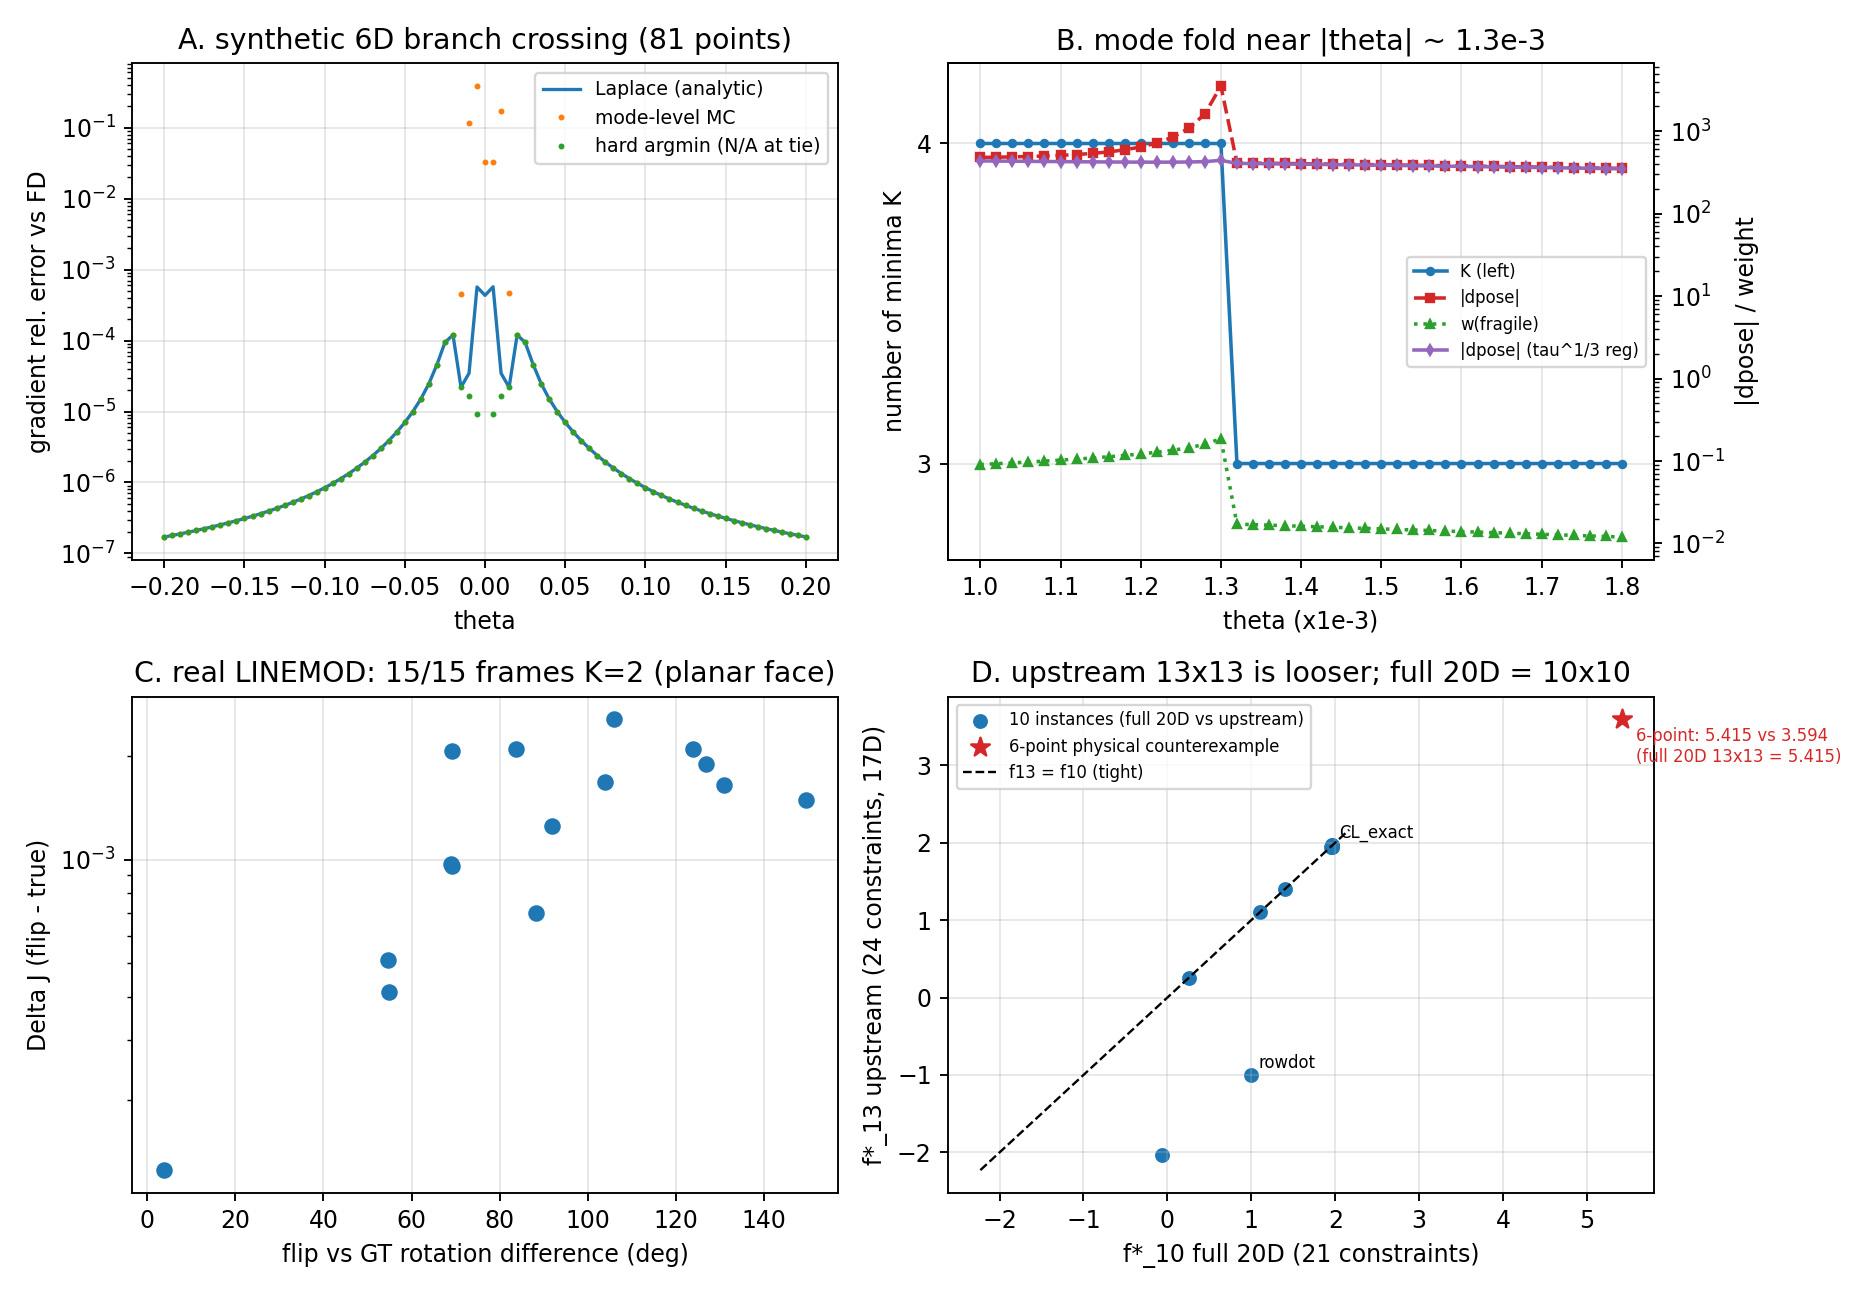
\includegraphics[width=0.92\textwidth]{p1_summary.png}
\caption{Overview of the four result families. \textbf{(A)} Gradient relative error vs $\theta$ on the 81-point synthetic 6D crossing for the analytic Laplace layer, the mode-level MC estimator and the hard argmin (N/A at the crossing); the Laplace curve has no jump, the hard map does. \textbf{(B)} The measured 6D fold near $|\theta|\sim1.3\times10^{-3}$: number of minima $K$, the pose-map jump $\|d\phi\|$ (standard and $\tau^{1/3}$-regularised) and the fragile-mode Laplace weight, all against $\theta$ on a $1.3\times10^{-3}$-scale axis; the mode dies at $\theta_f$ and $\|d\phi\|$ spikes there. \textbf{(C)} Real LINEMOD frames: the objective gap $\Delta J$ (flip minus true mode) against the flip-vs-GT rotation difference; all 15 frames have $K=2$. \textbf{(D)} Upstream 24-constraint $13\times13$ value against the full-20D $10\times10$ value on the 10 SDP instances and the 8 perturbations, with the six-point physical counterexample (star) separating the two: $5.415$ (full 20D) versus $3.594$ (upstream).}
\label{fig:p1summary}
\end{figure*}

\begin{table}[t]
\centering
\caption{Gradient relative error of the analytic Laplace layer, the mode-level MC baseline and the hard argmin, and the MC pose spread, per regime of the 81-point crossing grid ($\tau=0.01$, FD $h=10^{-4}$, mode-level MC $n=200$ with 20 seeds, CPU). Each entry is the median over the regime's grid points. The hard entry at $\theta=0$ is N/A because the global branch switches within $\pm h$.}
\label{tab:main6d}
\footnotesize
\setlength{\tabcolsep}{4pt}
\begin{tabular}{@{}l r l l l l@{}}
\toprule
regime & $n$ & Laplace & MC & hard & MC std\\
\midrule
far & 61 & 4.74e-07 & 4.74e-07 & 4.74e-07 & 2.76e-16\\
near & 19 & 3.46e-05 & 9.40e-05 & 2.23e-05 & 2.89e-16\\
at & 1 & 4.34e-04 & 3.26e-02 & N/A & 1.07e-01\\
\bottomrule
\end{tabular}
\end{table}

The grid has 61 far points, 19 near points and the single crossing point (nominal boundaries $|\theta|=0.05$ and $0.005$). Three observations follow.

\begin{enumerate}
\item \textbf{Away from the crossing the three methods coincide.} In the far regime all three median relative errors are $4.74\times10^{-7}$ and the median MC pose spread is $2.76\times10^{-16}$: the global mode carries essentially all of the Laplace mass and the sampler sees a single mode.
\item \textbf{The Laplace advantage is specific to the crossing.} In the near regime the hard argmin is still defined and has the smallest median error ($2.23\times10^{-5}$), ahead of Laplace and MC; the median MC spread is $2.89\times10^{-16}$, although the per-point maximum is $3.41\times10^{-2}$. At $\theta=0$ the hard entry is N/A, the Laplace entry is FD-limited (see below), and the MC error is $3.26\times10^{-2}$ with a pose spread of $1.07\times10^{-1}$.
\end{enumerate}

\textbf{The $4.34\times10^{-4}$ entry is FD truncation, not method error.} Against a Richardson-extrapolated FD it is $1.8\times10^{-7}$ at $\theta=0$, while against the plain central FD at $h=10^{-4}$ it is $4.3\times10^{-4}$; the sequence $4.34\times10^{-8}$ ($h=10^{-6}$), $4.34\times10^{-6}$ ($h=10^{-5}$), $4.34\times10^{-4}$ ($h=10^{-4}$) makes the same point. The near row is FD-limited for the same reason: at $\theta=0.01$ the study gives $3.46\times10^{-9}$ at $h=10^{-6}$ versus $3.46\times10^{-5}$ at $h=10^{-4}$. For $|\theta|\ge0.05$ the $h=10^{-5}$ error is at most $7.0\times10^{-8}$. The analytic gradient agrees with a Richardson FD to $1.8\times10^{-7}$ at the crossing, not to $4\times10^{-4}$.

\textbf{The hard argmin is a step map; the Laplace map is not.} The hard pose jump across $\theta=0$ stays $2.86$ as $\delta\to0$ ($\delta=10^{-3},10^{-4},10^{-5}$), while the Laplace jump decays linearly ($9.73\times10^{-1}$, $1.00\times10^{-1}$, $1.00\times10^{-2}$) with FD slope $\approx502$, i.e.\ the true derivative. Where its central FD is defined, the hard map is as self-consistent as Laplace (median $1.2\times10^{-4}$ over the non-switching cases), but it switches branch inside $\pm h$ in half of the exact-crossing cases. Fig.~\ref{fig:maintable} shows the per-point error and the MC spread.

\begin{figure}[t]
\centering
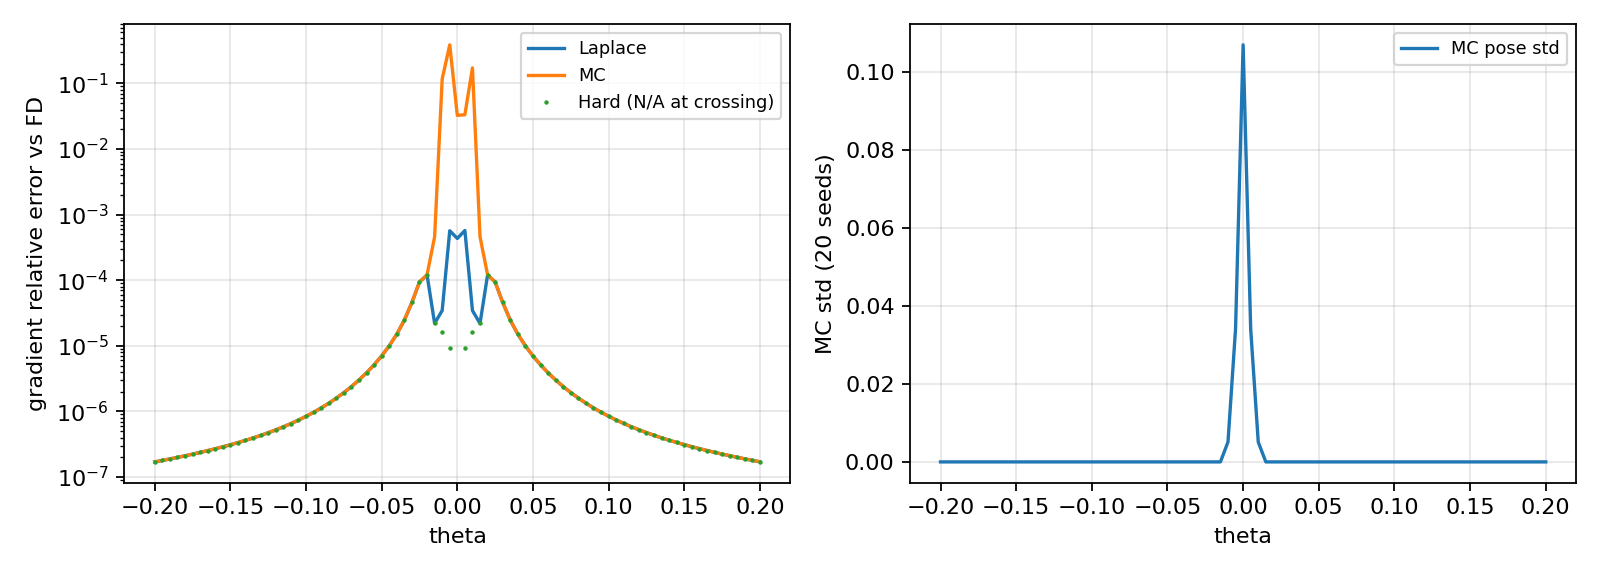
\includegraphics[width=\columnwidth]{main_table.png}
\caption{Main-table diagnostic on the 81-point 6D crossing grid. Left: gradient relative error against branch-following FD for the analytic Laplace layer (blue), the mode-level MC estimator (orange) and the hard argmin (green points; N/A at the exact crossing where the FD reference changes branch). Right: MC pose standard deviation over 20 seeds, which is essentially zero except in a narrow window around $\theta=0$.}
\label{fig:maintable}
\end{figure}

\textbf{The MC baseline is unbiased but noisy at a fixed budget.} On the same smoothed target, $n=200\times3$ seeds give a median per-seed gradient relative error of $0.05$ (20-seed mean $7.7\times10^{-3}$) and a median pose standard deviation of $0.09$ across the robustness conditions, versus $9.3\times10^{-8}$ for the analytic Laplace gradient against the Richardson reference. This is the measured variance cost of mode-level sampling.

\textbf{Mode count and fold.} The mode count over the grid is $K\in\{1,2,3,4\}$ ($K=1$ at 30 points, $K=2$ at 38, $K=3$ at 12, $K=4$ at the crossing point); these are the local minima returned by multi-start Newton with the filter above, not a certified root count. The smoothness statement is restricted to $\theta=0$ and $|\theta|\lesssim1.3\times10^{-3}$: a secondary minimum exists only there and disappears at the fold, where the Laplace map is discontinuous (Section~\ref{sec:fold6d}).

\subsection{1D exact posterior: the Laplace error is \texorpdfstring{$O(\tau)$}{O(tau)}}\label{sec:onepd}

\begin{table*}[t]
\centering
\caption{Exact posterior vs two-mode Laplace in the 1D normal form with unequal curvatures ($c=0.25$; at $g=0$ both minima sit at $x=\pm1$ with curvatures 5 and 3). $E$ is the posterior mean of $x$; errors are against a 2{,}000{,}001-point trapezoid on $[-3,3]$. Energies are dimensionless, and $\Delta J=6.16\times10^{-32}$ is numerical zero.}
\label{tab:1d}
\footnotesize
\setlength{\tabcolsep}{5pt}
\begin{tabular}{@{}l l l l l l l l@{}}
\toprule
regime & $\tau$ & $\Delta J$ & $E_{\mathrm{exact}}$ & $E_{\mathrm{Lap}}$ & $|{\rm err}|$ & $|{\rm err}|/\tau$ & rel grad err\\
\midrule
crossing & 0.05 & 6.16e-32 & -0.125102 & -0.127017 & 1.92e-03 & 3.83e-02 & 1.77e-02\\
crossing & 0.02 & 6.16e-32 & -0.126275 & -0.127017 & 7.42e-04 & 3.71e-02 & 6.93e-03\\
crossing & 0.01 & 6.16e-32 & -0.126649 & -0.127017 & 3.67e-04 & 3.67e-02 & 3.44e-03\\
crossing & 0.005 & 6.16e-32 & -0.126834 & -0.127017 & 1.83e-04 & 3.66e-02 & 1.71e-03\\
separated & 0.05 & 4.01e-01 & -1.024203 & -1.031750 & 7.55e-03 & 1.51e-01 & 2.77e-02\\
separated & 0.02 & 4.01e-01 & -1.029356 & -1.032296 & 2.94e-03 & 1.47e-01 & 1.27e-02\\
separated & 0.01 & 4.01e-01 & -1.030838 & -1.032296 & 1.46e-03 & 1.46e-01 & 6.27e-03\\
separated & 0.005 & 4.01e-01 & -1.031570 & -1.032296 & 7.26e-04 & 1.45e-01 & 3.12e-03\\
\bottomrule
\end{tabular}
\end{table*}

The expected-value error scales as $O(\tau)$: the log-log slope is 1.066 at the crossing and 1.036 in the separated basin, and $|{\rm err}|/\tau$ stays in $3.66$--$3.83\times10^{-2}$ at the crossing and $1.45$--$1.51\times10^{-1}$ when separated. The gradient error falls monotonically with $\tau$ on the printed rows; the gradient remainder is checked numerically rather than proved.

\subsection{Fold merging and the \texorpdfstring{$\tau^{1/3}$}{tau^(1/3)} regulariser}\label{sec:fold1d}

\begin{table*}[t]
\centering
\caption{Standard Laplace vs $\tau^{1/3}$-regularised volume factor at $\tau=0.01$, for $J=x^4/4-ax^2/2$; exact partition by a 2{,}000{,}001-point trapezoid on $[-3.5,3.5]$. $H=2a$ is the curvature at the minimum and the barrier is $a^2/4$.}
\label{tab:fold}
\scriptsize
\setlength{\tabcolsep}{2.5pt}
\begin{tabular}{@{}l l l l l l l l@{}}
\toprule
$a$ & $H$ & barrier & $Z_{\mathrm{exact}}$ & $Z_{\mathrm{Lap}}$ & rel err Lap & $Z_{\mathrm{reg}}$ & rel err reg\\
\midrule
0.50 & 1.00e+00 & 6.25e-02 & 2.6976e+02 & 2.5969e+02 & 3.73e-02 & 2.3556e+02 & 1.27e-01\\
0.20 & 4.00e-01 & 1.00e-02 & 2.3994e+00 & 2.1547e+00 & 1.02e-01 & 1.7371e+00 & 2.76e-01\\
0.10 & 2.00e-01 & 2.50e-03 & 1.2349e+00 & 1.4394e+00 & 1.66e-01 & 9.9871e-01 & 1.91e-01\\
0.05 & 1.00e-01 & 6.25e-04 & 9.7810e-01 & 1.6876e+00 & 7.25e-01 & 9.5017e-01 & 2.86e-02\\
0.02 & 4.00e-02 & 1.00e-04 & 8.6986e-01 & 2.5318e+00 & 1.91e+00 & 1.0019e+00 & 1.52e-01\\
0.01 & 2.00e-02 & 2.50e-05 & 8.3916e-01 & 3.5538e+00 & 3.24e+00 & 1.0358e+00 & 2.34e-01\\
\bottomrule
\end{tabular}
\end{table*}

As $a\to0$ the two minima and the saddle merge, $H\to0$, and the standard volume factor $1/\sqrt{H}$ diverges: the relative error grows from $3.73\times10^{-2}$ at $a=0.5$ to $1.91$ at $a=0.02$ and $3.24$ at $a=0.01$. Replacing $H$ by $H+\tau^{1/3}$ reduces the error to $1.52\times10^{-1}$ and $2.34\times10^{-1}$ at the two smallest $a$, but it is not uniformly better: at $a=0.5$ it is worse ($1.27\times10^{-1}$ versus $3.73\times10^{-2}$). The regularised form captures the $\tau^{1/3}$ scaling in the merging regime; it is not a drop-in replacement everywhere.

\subsubsection{The measured 6D fold}\label{sec:fold6d}

The 6D synthetic map has a genuine fold just off the crossing. A secondary minimum exists only for $|\theta|\lesssim1.3\times10^{-3}$ (the fine fold scan puts the mode death at $\theta_f=1.31\times10^{-3}$; the coarser robustness scan brackets it at $\approx1.4\times10^{-3}$); as it approaches the fold its $3\times3$ Hessian determinant falls through $3.35\times10^{-1}$ while its Laplace weight rises from $0.09$ to $0.187$ ($0.122$ at that determinant), and then the mode disappears ($K$ falls from 4 to 3). Across the fold the pose map steps by $0.31$ over one $2\times10^{-5}$ step (constant under grid refinement, i.e.\ a genuine discontinuity), and $\|d\phi\|$ peaks at $3529$ versus a median of $379$ away from the fold; the effective FD slope reaches $1.5\times10^4$. Neither a smaller $\tau$ nor more starts removes it: $n_{\rm starts}\ge32$ matches the 1024-start median $K$ (64 starts reproduce the full mode set on the sweep), while $n_{\rm starts}=16$ misses the fragile mode in 10\% of independent draws and a miss moves the pose by up to 28\% and the gradient by up to 97\%. The smoothness and $O(\tau)$ accuracy statements are therefore restricted to $\theta=0$ and $|\theta|\lesssim1.3\times10^{-3}$; the multi-modal Laplace map is discontinuous where a minimum is born or dies.

\textbf{A partial fix for the fold.} Replacing $\det H$ by $\det(H+\epsilon I)$ with $\epsilon=\tau^{1/3}$ (the 1D rule above, whose derivative is still closed form, $\operatorname{tr}((H+\epsilon I)^{-1}\dot H)$) largely removes the \emph{derivative} singularity: at $\theta=1.30\times10^{-3}$ the standard $\|d\phi\|$ is $3529$ while the regularised one is $443$, and the near-fold gradient error falls from $2.90\times10^{-1}$ to $1.19\times10^{-2}$ (a factor 24); away from the fold ($\theta=0.1,0.02$) the two variants agree to the printed precision. It does not remove the \emph{value} discontinuity caused by a minimum dying: the pose step across the fold only falls from $0.309$ to $0.107$ and $K$ still changes from 4 to 3. Hessian regularisation is therefore a cheap mitigation for the fold neighbourhood; a continuity claim across the fold requires the Scorer continuation of Section~\ref{sec:discussion} or a local numerical integral over the merging pair.

\subsection{Rotation-SDP certificate and the three-part \texorpdfstring{$10\times10$/$13\times13$}{10x10/13x13} relation}\label{sec:results_sdp}

\begin{table}[t]
\centering
\caption{Numerical certificate for the constructed $10\times10$ rotation SDP (Choi--Lam quartic plus $2I$; SCS). The gap is $f^\star-\mu$, where $f^\star=2$ is the analytic minimum of the quartic on $\mathbb{S}^3$ and $\mu$ is the certified dual value.}
\label{tab:sdp_cert}
\scriptsize
\setlength{\tabcolsep}{3pt}
\begin{tabular}{@{}p{4.6cm} l@{}}
\toprule
quantity & value\\
\midrule
$f^\star$ (analytic, $C\ge0$, $C(e_0)=0$) & 2.0\\
SDP primal value & 1.9658119658\\
dual $\mu$ & 1.9658119658\\
$\lambda_{\min}(Z)$ of the dual certificate & $-1.79\times10^{-11}$\\
certified gap $f^\star-\mu$ & 0.034188\\
$\operatorname{rank}(X^\star)$ at tolerance $10^{-6}$ & 6\\
$\lambda_1/\lambda_2$ & 1.451\\
multi-start QPEP minimum (independent check) & 2.00186\\
random perturbations with positive gap & 8 of 8 (0.0453--0.0782)\\
rank of the 21 $SO(3)$ constraints & 20\\
dimension of the degree-two vanishing ideal & 20\\
\bottomrule
\end{tabular}
\end{table}

The primal value, dual value and gap of the $10\times10$ instance are mutually consistent to the printed digits; the gap is $0.034188034\ldots$. This is our own construction (Example~\ref{ex:choilam}). Theorem~\ref{thm:thirteen} gives the three-part relation to the released $13\times13$ implementation, and the measurements below instantiate each layer.

\begin{table*}[t]
\centering
\caption{The upstream 24-constraint $13\times13$ relaxation is strictly looser in general than the full-20D $10\times10$ relaxation. $f^\star_{10}$ is the $10\times10$ value and $f^\star_{13,\mathrm{up}}$ the value of the released implementation (17-dimensional span); \texttt{CL\_exact} is the constructed Choi--Lam instance and \texttt{rowdot} the constructed counterexample. For \texttt{CL\_exact} and \texttt{p6\_data} the true differences are $3.7\times10^{-11}$ and $-2.9\times10^{-10}$, below the six-digit columns.}
\label{tab:13v10}
\footnotesize
\setlength{\tabcolsep}{6pt}
\begin{tabular}{@{}l l l l l l@{}}
\toprule
instance & $f^\star_{10}$ & $f^\star_{13,\mathrm{up}}$ & $f^\star_{10}-f^\star_{13,\mathrm{up}}$ & rank $X_{10}^\star$ & rank $X_{13,\mathrm{up}}^\star$\\
\midrule
\texttt{CL\_exact} & 1.965812 & 1.965812 & 3.7e-11 & 6 & 6\\
\texttt{CL\_pert0} & 1.962860 & 1.960078 & 2.8e-03 & 6 & 5\\
\texttt{CL\_pert5} & 1.964571 & 1.950275 & 1.4e-02 & 6 & 4\\
\texttt{rowdot} & 1.000000 & -1.000000 & 2.00 & 10 & 7\\
\texttt{rowdot\_gen} & -0.060192 & -2.029230 & 1.97 & 1 & 4\\
\texttt{p6\_data} & 0.252326 & 0.252326 & 0.0 & 1 & 1\\
\bottomrule
\end{tabular}
\end{table*}

\textbf{Interpretation.} The Choi--Lam equality is a coincidence of symmetry: its upstream optimum lies on the row-orthogonality face, so $f^\star_{13,\mathrm{up}}=f^\star_{10}=1.9658119658$ with rank 6 on both sides and a row-dot residual at most $8.8\times10^{-15}$. After eight symmetry-breaking perturbations of order $10^{-2}$, $8/8$ instances have $f^\star_{13,\mathrm{up}}<f^\star_{10}$ by $2.5\times10^{-3}$--$1.4\times10^{-2}$, with $\operatorname{rank}(X^\star_{13,\mathrm{up}})\in\{4,5\}$ against $\operatorname{rank}(X^\star_{10})=6$, and $\max|r_a\cdot r_b|$ at the upstream optimum is $0.59$--$0.88$. The constructed objective $Q=-r_1\cdot r_2+\tfrac14I$ isolates the mechanism: it is the constant 1 on the full-20D feasible set ($f^\star_{10}=1.000000$), while upstream it reaches $-1.000000$ (gap $2.00$), and still $1.97$ after a $10^{-2}$ perturbation. These measurements instantiate layer (2), not layer (1), of Theorem~\ref{thm:thirteen}.

\begin{table}[t]
\centering
\caption{6-point physical 3D--3D counterexample separating the upstream $13\times13$ relaxation from the full-20D one. Construction: $p_i=\pm e_1,\pm e_2,\pm e_3$ and $y_i=\varepsilon p_i$ with $\varepsilon=0.05$, shared matrix weights $W$ with $W_{11}=W_{22}=W_{33}=1$ and $W_{12}=W_{21}=-0.6$ (eigenvalues $0.4,1.0,1.6>0$), $N=6$, so $D=0$ and $G=6W\succ0$; the ground-truth rotation $R^\star=I_3$ is unique. The middle rank follows from layer (1); the analytic column states ranks 1 and 4 explicitly.}
\label{tab:6point}
\scriptsize
\setlength{\tabcolsep}{3pt}
\begin{tabular}{@{}p{4.1cm} l l@{}}
\toprule
quantity & numerical & analytic\\
\midrule
$f^\star_{10}$ (21 constraints, exact rank 20) & 5.41500000 & 5.41500000\\
$f^\star_{13,\mathrm{full}}$ (24 + 3 row-orthogonality = 27 constraints, full 20D) & 5.41500000 & 5.41500000\\
$f^\star_{13,\mathrm{up}}$ (24 constraints, 17D span) & 3.59431373 & 3.59430886\\
$f^\star_{10}-f^\star_{13,\mathrm{up}}$ & 1.82068627 & 1.82069114\\
ranks of $X^\star_{10}$ / $X^\star_{13,\mathrm{full}}$ / $X^\star_{13,\mathrm{up}}$ & 1 / 1 / 4 & 1 / 1 / 4\\
$f_{\rm nonconv}-f^\star_{10}$ & $-8.38\times10^{-13}$ & 0\\
$f_{\rm nonconv}-f^\star_{13,\mathrm{full}}$ & $-3.38\times10^{-13}$ & 0\\
$f_{\rm nonconv}-f^\star_{13,\mathrm{up}}$ & 1.820686 & 1.820691\\
\bottomrule
\end{tabular}
\end{table}

\textbf{Why this instance separates the two.} With $\pm p_i$ cancelling pairwise, $D=\mathbf{0}$, and the cost is
\begin{equation}
J(R,t)=2\,\mathrm{tr}(WRR^\top)-4\varepsilon\,\mathrm{tr}(WR)+2\varepsilon^2\mathrm{tr}(W)+6t^\top Wt .
\label{eq:sixpoint}
\end{equation}
The only term that sees row orthogonality is $2\,\mathrm{tr}(WRR^\top)=2(\|r_1\|^2+\|r_2\|^2+\|r_3\|^2-1.2\,r_1^\top r_2)$. Under the full-20D constraints $r_1^\top r_2=0$ makes it the constant $6$, and $-4\varepsilon\,\mathrm{tr}(WR)$ is minimised at $R=I$ with value $6(1-\varepsilon)^2=5.415$, so $f^\star_{10}=f^\star_{13,\mathrm{full}}=f^\star_{\mathrm{QPEP}}=5.41500000$ with rank 1 and gap zero at SCS level. Upstream, the missing $r_1^\top r_2=0$ lets the relaxation take $\langle r_1^\top r_2\rangle>0$ and drop to $f^\star_{13,\mathrm{up}}=3.59431373$ with rank 4.

\textbf{The $4.9\times10^{-6}$ difference in the analytic column.} SCS ($\varepsilon=10^{-11}$) gives $3.59431373$ and CLARABEL gives $3.59431371$ (agreement $2\times10^{-8}$), and an exact-rational dual certificate (exact rational LDU with $\eta=10^{-11}$; minimum pivot $1.0\times10^{-11}$, mpmath 60-digit $\lambda_{\min}=+8.0\times10^{-12}$) yields the rigorous lower bound $f^\star_{13,\mathrm{up}}\ge3.594313732834$. The analytic value $3.59430886$ lies $4.87\times10^{-6}$ \emph{below this bound}, so it cannot be the optimum of the stated 24-constraint SDP; 36 natural variants (scaling, subsets, layout, normalisation, $t$ block and solver tolerances) do not reproduce it within $10^{-8}$, the closest being $4.1\times10^{-6}$ away. The solver value $3.5943137\ldots$ with gap $1.8206863\ldots$ is consistent with the bound. The qualitative separation (gap $1.82$, rank $1$ versus $>1$) is unaffected, and $\operatorname{rank}(X^\star_{13,\mathrm{up}})$ is $4$ at a $10^{-5}$ threshold and $6$ at $10^{-6}$. Because this is a genuine matrix-weighted 3D--3D cost, the Choi--Lam realizability question does not apply: the gap is a property of the released constraint set, and the three missing row-orthogonality constraints are the entire cause.

\subsection{Derivative checks and the root count}\label{sec:rootcount}

\begin{table}[t]
\centering
\caption{Numerical checks of the backward pass and of the closed-form $\partial_\theta\log\det H$. All entries are relative errors unless marked absolute.}
\label{tab:backward}
\scriptsize
\setlength{\tabcolsep}{3pt}
\begin{tabular}{@{}p{3.85cm} p{3.9cm}@{}}
\toprule
check & value\\
\midrule
$E(q)$ orthonormal error & 1.14e-16\\
$E(q)^\top q$ error & 4.41e-18\\
Euler identity absolute error & 5.33e-15\\
Riemannian Hessian, analytic vs FD & 9.63e-08\\
implicit $\partial q^\star/\partial\theta$ vs FD & 1.51e-07\\
implicit $\partial t^\star/\partial\theta$ vs FD & 4.58e-08\\
antipodal errors ($E$, $H$, $\partial q^\star$, $\partial R$) & 0 (exact)\\
Laplace integral rel. error (chart on $S^3$), $\tau=0.2/0.1/0.05/0.025$ & 8.26e-02 / 3.81e-02 / 1.86e-02 / 9.25e-03\\
log-log slope of Laplace error vs $\tau$ & 1.05\\
closed-form $\partial_\theta\log\det H$ vs FD, 5 trials & 1.65e-09 -- 8.84e-09\\
\quad (max abs err) & 1.59e-09\\
closed-form \texttt{dlogdetH\_dtheta} vs \texttt{dlogdet\_exact}, after fix & 8.9e-16\\
closed-form \texttt{dlogdetH\_dtheta} vs branch FD, after fix & 1.8e-9\\
regression test: \texttt{dE}/\texttt{dH}/\texttt{dq} & 2.9e-11 / 1.6e-8 / 2.5e-10\\
\bottomrule
\end{tabular}
\end{table}

The backward-pass checks confirm Theorem~\ref{thm:implicit} to FD accuracy; they do not certify the root set. The Laplace-constant check gives a slope of 1.05, consistent with the $O(\tau)$ claim of Theorem~\ref{thm:laplace} and inconsistent with an exact rotation integral. The closed-form $\log\det$ derivative matches the independent exact derivative to $8.9\times10^{-16}$ and branch FD to $1.8\times10^{-9}$, and matches FD to $9\times10^{-9}$ or better on all five trials; the regression pins \texttt{dE}/\texttt{dH}/\texttt{dq} at $2.9\times10^{-11}$/$1.6\times10^{-8}$/$2.5\times10^{-10}$.

\textbf{Root count and enumeration.} A total-degree homotopy on the projective stationarity system, run in all four affine charts with a batched complex predictor--corrector and residual-verified union, finds \textbf{40 complex projective roots on 4/4 instances}---three random symmetric $M$ and the 6D instance $M(0)$---with maximum chart residual $7.1\times10^{-15}$ and 5.3--8.0 s per instance. Each projective root corresponds to 80 affine roots with the $\pm$ double cover. The real picture varies: real projective roots $26/12/12/20$, real local minima $5/2/2/4$; the complex count is generic (the QPEP action-matrix bound of 40) and the real count is an instance property. This confirms the ``at most 40 candidate complex roots'' of Section~\ref{sec:cert} and certifies the algebraic system, but not the multi-start Newton enumerator used in E1/E8. That enumerator is exact only up to assumption (A2): against a 1024-start reference, $n_{\rm starts}\ge64$ reproduces the mode set on the sweep and $32$ matches the median $K$, while $n_{\rm starts}=16$ misses the fragile mode in 10\% of independent draws, so the mode counts of Section~\ref{sec:synthetic} are lower bounds on the true count.\label{sec:enumeration}

\subsection{Ablations}\label{sec:ablations}

\textbf{A. Temperature.} Table~\ref{tab:tau} reports the gradient relative error of the exact-logdet Laplace layer for $\tau\in\{0.05,0.02,0.01,0.005\}$ at the crossing, near the crossing, and far from it.

\begin{table}[t]
\centering
\caption{$\tau$ sweep (gradient relative error).}
\label{tab:tau}
\footnotesize
\setlength{\tabcolsep}{4pt}
\begin{tabular}{@{}l l l l l@{}}
\toprule
$\theta$ & $\tau=0.05$ & 0.02 & 0.01 & 0.005\\
\midrule
+0.000 & 1.20e-03 & 5.84e-04 & 4.34e-04 & 1.51e-03\\
+0.010 & 1.29e-05 & 1.07e-04 & 3.46e-05 & 1.64e-05\\
-0.010 & 1.29e-05 & 1.06e-04 & 3.46e-05 & 1.63e-05\\
+0.100 & 8.47e-07 & 8.46e-07 & 8.46e-07 & 8.46e-07\\
-0.100 & 8.43e-07 & 8.42e-07 & 8.42e-07 & 8.42e-07\\
\bottomrule
\end{tabular}
\end{table}

At the crossing the error is smallest at $\tau=0.01$ and rises again at $\tau=0.005$, consistent with the FD reference becoming unreliable when the two modes are nearly degenerate; far from the crossing it is $\approx8.5\times10^{-7}$ and independent of $\tau$.

\textbf{B. Volume factor.} Table~\ref{tab:volume} compares the closed-form $\log\det$ derivative, a tangent-space FD, and dropping the volume factor from the weights.

\begin{table}[t]
\centering
\caption{Volume-factor variants. \texttt{exact} is the closed form of Section~\ref{sec:laplace}, \texttt{numeric} is a tangent-space FD, \texttt{none} drops $\tfrac12\log\det H_k$ from the weights; \emph{pose diff} and \emph{grad diff} are Euclidean norms of the differences in the 12-vector against \texttt{exact}.}
\label{tab:volume}
\scriptsize
\setlength{\tabcolsep}{3pt}
\begin{tabular}{@{}l l l l l@{}}
\toprule
$\theta$ & mode & grad rel & pose diff & grad diff\\
\midrule
+0.000 & exact & 4.34e-04 & 0.00e+00 & 0.00e+00\\
+0.000 & numeric & 4.34e-04 & 0.00e+00 & 2.22e-08\\
+0.000 & none & 3.75e-04 & 6.47e-02 & 5.34e+01\\
+0.010 & exact & 3.46e-05 & 0.00e+00 & 0.00e+00\\
+0.010 & numeric & 3.46e-05 & 0.00e+00 & 1.22e-11\\
+0.010 & none & 3.86e-05 & 7.77e-04 & 4.38e-01\\
-0.010 & exact & 3.46e-05 & 0.00e+00 & 0.00e+00\\
-0.010 & numeric & 3.46e-05 & 0.00e+00 & 1.89e-11\\
-0.010 & none & 3.86e-05 & 7.79e-04 & 4.39e-01\\
\bottomrule
\end{tabular}
\end{table}

Dropping the volume factor leaves the gradient relative error almost unchanged at the crossing but changes the smoothed pose by $6.47\times10^{-2}$ and the gradient by $5.34\times10^{1}$ in absolute norm; near the crossing the gradient changes by $0.44$. The factor is therefore not cosmetic for the smoothed map, and the closed form and the tangent-space FD agree to $2.22\times10^{-8}$ or better.

\textbf{C. Top-$K$ mode truncation.} Table~\ref{tab:topk} keeps only the $K$ highest-weight modes and compares the result with the sum over all modes.

\begin{table}[t]
\centering
\caption{Top-$K$ mode truncation (reference: all modes).}
\label{tab:topk}
\footnotesize
\setlength{\tabcolsep}{4pt}
\begin{tabular}{@{}l l l l@{}}
\toprule
$\theta$ & $K$ & pose diff & grad diff\\
\midrule
+0.000 & 1 & 1.44e+00 & 4.99e+02\\
+0.000 & 2 & 1.05e-01 & 6.83e+01\\
+0.000 & 3 & 7.95e-02 & 4.93e+01\\
+0.000 & 4 & 0.00e+00 & 0.00e+00\\
+0.010 & 1 & 2.72e-03 & 1.98e+00\\
+0.010 & 2 & 3.02e-05 & 2.65e-02\\
+0.010 & 3 & 0.00e+00 & 0.00e+00\\
+0.010 & 4 & 0.00e+00 & 0.00e+00\\
\bottomrule
\end{tabular}
\end{table}

At $\theta=0$, keeping only the top mode changes the pose by $1.44$ and the gradient by $499$ relative to the all-mode sum, while $K=2$ cuts these to $0.105$ and $68.3$; at $\theta=0.01$, $K=3$ is already exact. Summing over all enumerated minima is therefore necessary at a tie, although the number of modes a real cost carries remains an instance property.

\subsection{Real two-mode cost on LINEMOD}\label{sec:real}

Part A builds the cost on the dominant planar face selected by deterministic RANSAC. A planar target has the classical two-fold pose ambiguity, so the bearing cost has two genuine minima; modes whose transformed points fall behind the camera ($z\le0$) are rejected. An earlier variant that mixed two full costs under a single shared translation produced no usable rows; giving each hypothesis its own translation, as in Part B, removes the compromise pose.

\begin{table*}[t]
\centering
\caption{Real two-mode bearing cost on the dominant planar face (Part A). All 15 frames have $K_{\rm phys}=2$ physical minima ($K_{\rm all}=4$ before the $z>0$ filter). $w({\rm other})$ is the Laplace weight of the physical mode that is not the hard argmin (the flip in 14/15 frames; the GT-like mode in \texttt{000010/72}). Rotation errors are in degrees against BOP ground truth; the Laplace entry is the projected chordal mean $\mathrm{Proj}_{SO(3)}(\sum_kw_kR_k)$.}
\label{tab:twomode}
\scriptsize
\setlength{\tabcolsep}{4pt}
\begin{tabular}{@{}l r r l r r r r@{}}
\toprule
frame/img & obj & $n_{\rm plane}$ & $\Delta J$ & other-mode (deg) & $w({\rm other})$ & hard rot err (deg) & Laplace rot err (deg, projected)\\
\midrule
000010/15 & 10 & 558 & 9.58e-04 & 69.3 & 0.483 & 1.47 & 33.90\\
000010/18 & 10 & 474 & 1.25e-03 & 91.9 & 0.472 & 0.51 & 42.85\\
000010/40 & 10 & 482 & 9.71e-04 & 69.1 & 0.482 & 2.20 & 33.07\\
000010/60 & 10 & 452 & 1.69e-03 & 104.0 & 0.459 & 0.96 & 46.45\\
000010/66 & 10 & 460 & 7.00e-04 & 88.4 & 0.488 & 2.29 & 43.67\\
000010/72 & 10 & 501 & 1.25e-04 & 3.8 & 0.504 & 44.46 & 23.02\\
000010/80 & 10 & 508 & 5.11e-04 & 54.7 & 0.501 & 1.08 & 27.71\\
000010/90 & 10 & 474 & 4.13e-04 & 54.8 & 0.497 & 3.49 & 27.91\\
000011/20 & 11 & 413 & 2.07e-03 & 69.1 & 0.608 & 8.14 & 44.24\\
000011/24 & 11 & 423 & 1.65e-03 & 131.1 & 0.457 & 1.37 & 54.99\\
000011/26 & 11 & 439 & 1.90e-03 & 126.9 & 0.450 & 2.06 & 51.65\\
000011/32 & 11 & 474 & 2.10e-03 & 123.9 & 0.451 & 1.78 & 51.60\\
000011/33 & 11 & 365 & 1.49e-03 & 149.6 & 0.460 & 1.62 & 59.09\\
000011/40 & 11 & 428 & 2.56e-03 & 106.0 & 0.457 & 2.77 & 46.19\\
000011/49 & 11 & 347 & 2.10e-03 & 83.7 & 0.528 & 4.95 & 46.75\\
\bottomrule
\end{tabular}
\end{table*}

\begin{figure}[t]
\centering
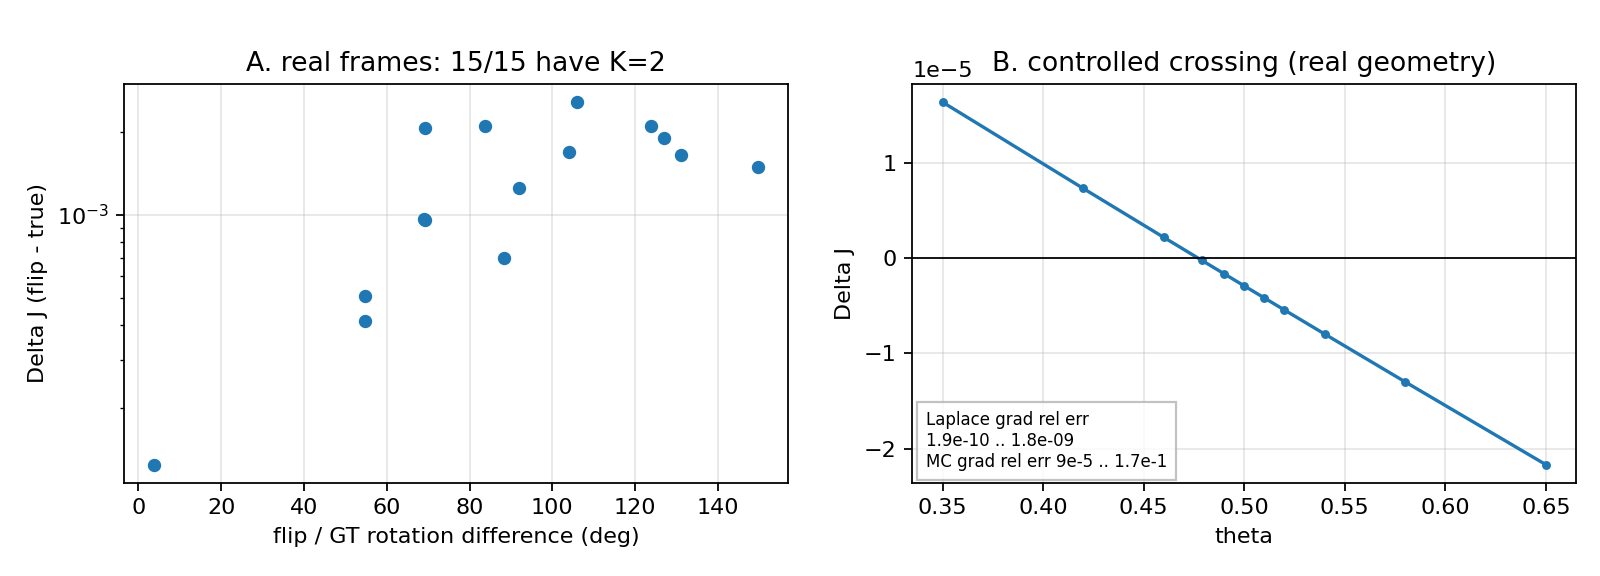
\includegraphics[width=\columnwidth]{two_mode.png}
\caption{The real two-mode cost. Left: for each of the 15 LINEMOD frames, the objective gap $\Delta J$ between the flip and the GT-like mode against the angle between the two modes; every frame has $K_{\rm phys}=2$, with $\Delta J\in[1.25\times10^{-4},2.56\times10^{-3}]$. Right: the controlled transverse crossing on real geometry (Part B), where the two labelled hypotheses are mixed as $J_\theta=(1-\theta)J_{\rm true}+\theta J_{\rm sym}$; $\Delta J$ changes sign near $\theta\approx0.475$. The inset reports the analytic Laplace gradient error against central FD ($1.9\times10^{-10}$--$1.8\times10^{-9}$) and the 400-sample MC error ($9\times10^{-5}$--$1.7\times10^{-1}$).}
\label{fig:twomode}
\end{figure}

Three points follow. First, the two-mode structure is reproducible: $K_{\rm phys}=2$ in 15/15 frames, with $\Delta J\in[1.25\times10^{-4},2.56\times10^{-3}]$, other-mode angles $3.8^\circ$--$149.6^\circ$ and $w({\rm other})=0.450$--$0.608$. Second, the GT-like mode is the lowest-$J$ physical mode in 14/15 frames, so the hard argmin is accurate: median rotation error $2.06^\circ$ $[1.47,3.49]$ and median ADD-S $3.7$ mm $[3.0,4.3]$, with one failure above $10^\circ$ (\texttt{000010/72}, $44.5^\circ$). Third, the Laplace posterior mean is not an accuracy win on these near-ties: median projected rotation error $44.24^\circ$ $[33.90,46.87]$, paired bias $+36.9^\circ$ $[+27.2,+44.9]$, median ADD-S $13.9$ mm $[10.3,20.2]$, i.e.\ roughly half the mass on the flip. The smallest Hessian determinant is $6.09\times10^{-3}$ (\texttt{000011/20}), so the flip mode is itself close to a fold.

\begin{table*}[t]
\centering
\caption{Aggregate pose error and ADD-S on the 15 real frames. Medians with 95\% percentile-bootstrap CIs over frames (1000 resamples). The paired bias is the mean per-frame difference against the hard argmin (95\% CI over frames); the median paired rotation bias is $+41.8^\circ$. ``Within $10^\circ$'' counts frames whose estimate is within $10^\circ$ of GT; for the posterior mean this is not a ``true mode'', since the mean need not be a mode.}
\label{tab:aggregate}
\scriptsize
\setlength{\tabcolsep}{3.5pt}
\begin{tabular}{@{}l l l l l l l@{}}
\toprule
method & rot med (deg) & ADD-S med (mm) & ADD med (mm) & rot bias (deg) & ADD-S bias (mm) & $\le10^\circ$ / true mode\\
\midrule
hard argmin & 2.06 [1.47, 3.49] & 3.7 [3.0, 4.3] & 5.9 [5.2, 11.1] & --- & --- & 14/15 true mode\\
Laplace (projected) & 44.24 [33.90, 46.87] & 13.9 [10.3, 20.2] & 38.1 [31.0, 41.5] & +36.9 [+27.2, +44.9] & +9.4 [+6.4, +12.6] & 0/15\\
MC (20 seeds) & 43.80 [33.90, 47.43] & 14.1 [10.3, 20.0] & 38.0 [31.0, 41.5] & +37.2 [+26.7, +45.0] & +9.4 [+6.4, +12.5] & 0/15\\
\bottomrule
\end{tabular}
\end{table*}

\begin{figure*}[t]
\centering
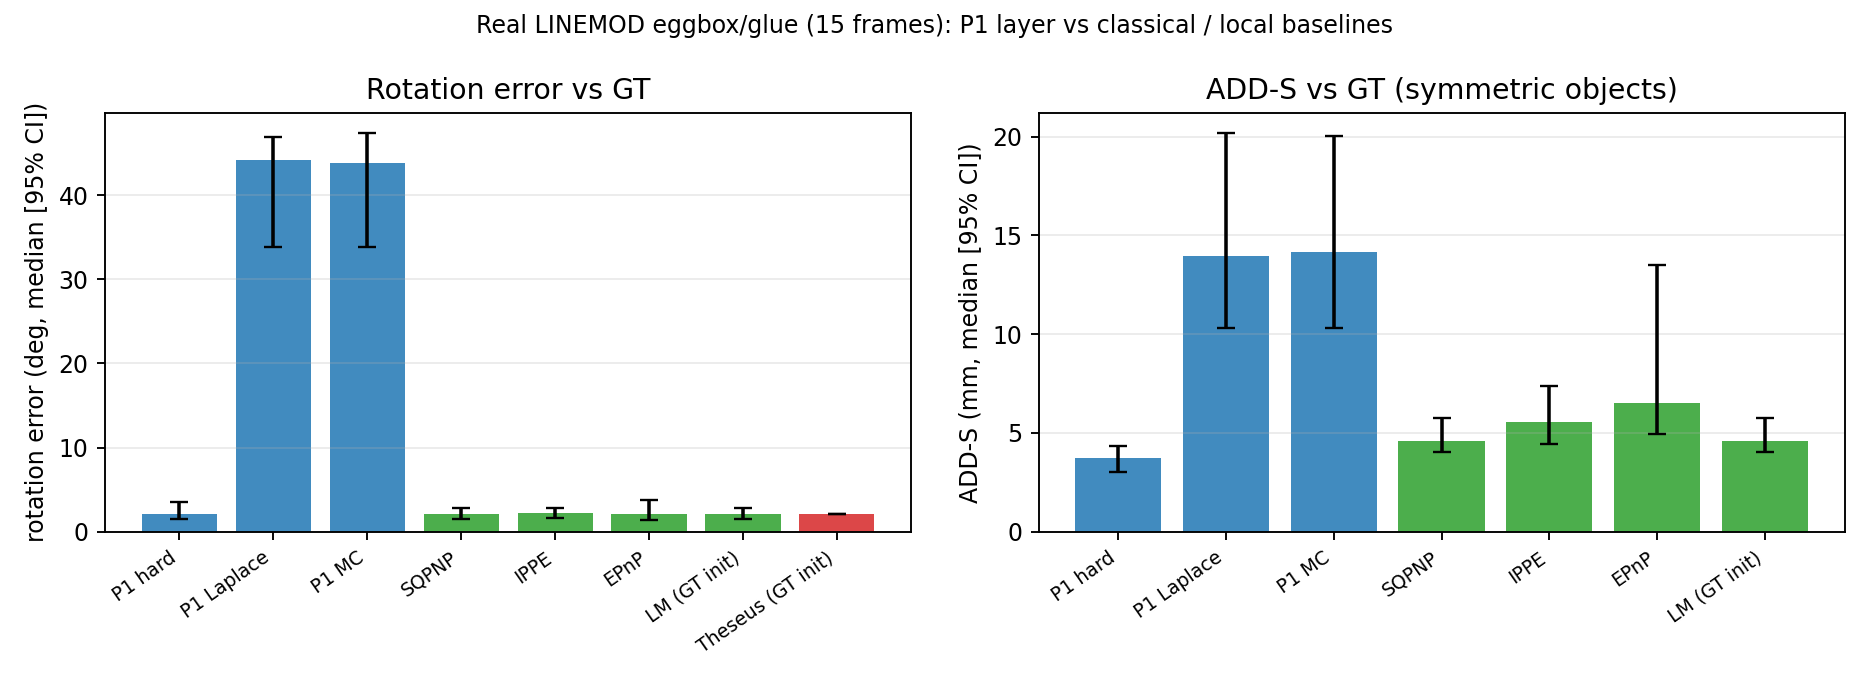
\includegraphics[width=\textwidth]{real_summary.png}
\caption{Real LINEMOD \texttt{eggbox}/\texttt{glue} results on the 15 frames, medians with 95\% bootstrap CIs. Left: rotation error against BOP ground truth for the P1 layer (hard argmin, projected Laplace mean, 20-seed MC) and for the forward/local references (SQPNP, IPPE, EPnP, local LM from GT init, Theseus from GT init). Right: ADD-S for the same methods (Theseus is not plotted). The hard argmin is at the classical-solver level; both posterior-mean estimates sit near $44^\circ$ because they average the two modes. Green bars are forward/local references; the red bar is a local solver started at ground truth and is not a deployable baseline.}
\label{fig:realsummary}
\end{figure*}

The 15-frame aggregates are in Table~\ref{tab:aggregate}. Means exceed medians for the hard argmin ($5.28^\circ$, $6.0$ mm) because of the single failure frame, while the Laplace means are $42.21^\circ$ and $15.5$ mm; translation medians are $6.2$ mm (hard) and $20.2$ mm (Laplace). MC estimates the same smooth mean ($0.23^\circ$ from the Laplace aggregate, within its seed-level CI) and inherits the bias, adding only seed noise (between-seed SD $1.011^\circ$).

\begin{table}[t]
\centering
\caption{Per-frame ADD-S (mm) and ADD reference (mm) on the 15 real frames. ADD-S is the primary object-space metric; ADD is same-index distance and is not invariant to the objects' $\sim180^\circ$ symmetry.}
\label{tab:perframe}
\scriptsize
\setlength{\tabcolsep}{2.5pt}
\begin{tabular}{@{}l r l l l l@{}}
\toprule
frame/img & obj & ADD-S hard & ADD-S Lap & ADD-S MC & ADD Lap (ref)\\
\midrule
000010/15 & 10 & 3.0 & 10.3 & 10.3 & 31.0\\
000010/18 & 10 & 4.3 & 12.2 & 12.3 & 37.6\\
000010/40 & 10 & 6.2 & 9.7 & 9.7 & 31.1\\
000010/60 & 10 & 3.0 & 13.9 & 14.1 & 40.7\\
000010/66 & 10 & 2.7 & 12.1 & 12.0 & 38.0\\
000010/72 & 10 & 12.5 & 8.4 & 8.4 & 22.3\\
000010/80 & 10 & 3.8 & 8.8 & 8.9 & 24.1\\
000010/90 & 10 & 3.1 & 8.5 & 8.4 & 23.3\\
000011/20 & 11 & 13.8 & 22.9 & 22.8 & 72.7\\
000011/24 & 11 & 2.8 & 20.2 & 20.0 & 40.5\\
000011/26 & 11 & 3.7 & 17.6 & 17.5 & 38.1\\
000011/32 & 11 & 3.1 & 19.0 & 19.0 & 41.5\\
000011/33 & 11 & 3.8 & 23.4 & 23.7 & 41.5\\
000011/40 & 11 & 2.2 & 16.8 & 16.7 & 44.7\\
000011/49 & 11 & 22.4 & 28.1 & 28.2 & 75.9\\
\bottomrule
\end{tabular}
\end{table}

Two per-frame readings matter. (i) On \texttt{000010/72} the hard argmin is the mode $44.5^\circ$ from GT while the GT-like mode is $3.8^\circ$ away but higher in $J$ by $1.25\times10^{-4}$; Laplace/MC land between the modes ($23.0^\circ$, $8.4$ mm) and are closer than the hard failure. That is a single-frame accident of the loss ranking, not evidence that the posterior mean is more accurate in general. (ii) ADD is $2$--$3\times$ ADD-S for the Laplace pose (median $38.1$ vs $13.9$ mm) because the glue object is long and thin and the $\sim180^\circ$ symmetry relabels it; this is why ADD-S, not ADD, is the reported metric.

\subsubsection{Classical forward solvers on the same correspondences}\label{sec:classical}

Table~\ref{tab:classical} runs cv2's EPnP, ITERATIVE, SQPNP and IPPE, plus a plain local GN/LM on the same bearing cost, on the bitwise-identical 15-frame correspondences (verified bitwise identical across the two studies; the GT-pose re-projection residual is $1.47$ px median, i.e.\ the $\sim1$ px nearest-vertex quantisation). These are forward solvers, not differentiable layers: the LM is a plain forward optimiser on the same cost, not BPnP, and no gradient claim is attached to any of them. IPPE is run on the RANSAC inliers projected onto the fitted plane (it requires exact coplanarity, planarity RMS $0.83$--$1.47$ mm); the other solvers use the raw inliers.

\begin{table*}[t]
\centering
\caption{Classical forward PnP baselines on the 15 real frames. Median with 95\% bootstrap CI over frames (2000 resamples). ``True mode'' counts solutions within $10^\circ$ of GT. SQPNP returns one solution in cv2 5.0.0 (documented for non-P3P/IPPE flags and observed on all 15 frames); IPPE returns two planar solutions, and the first (cheapest-reprojection) one is the GT-closer one on all 15 frames, so the oracle row would be identical to ``IPPE first''.}
\label{tab:classical}
\scriptsize
\setlength{\tabcolsep}{4pt}
\begin{tabular}{@{}l l l l@{}}
\toprule
method & rot median [CI] (deg) & ADD-S median [CI] (mm) & true mode\\
\midrule
EPnP & 2.05 [1.41, 3.71] & 6.5 [5.0, 13.5] & 12/15\\
ITERATIVE (homography init + LM) & 2.07 [1.60, 3.54] & 6.5 [5.7, 8.7] & 11/15\\
SQPNP (1 solution) & 2.04 [1.47, 2.77] & 4.6 [4.0, 5.8] & 15/15\\
IPPE (first, plane-projected) & 2.21 [1.68, 2.76] & 5.5 [4.4, 7.4] & 15/15\\
local LM, identity init & 106.01 [69.14, 179.82] & 40.7 [28.0, 1708.7] & 3/15\\
local LM, GT init & 2.06 [1.47, 2.77] & 4.6 [4.0, 5.8] & 15/15\\
local LM, flip init & 88.39 [69.08, 106.01] & 23.5 [16.9, 28.0] & 0/15\\
\bottomrule
\end{tabular}
\end{table*}

The ADD-S column here uses the 1000-query/1000-GT-vertex estimator, which carries a $+1.1$ mm discretisation floor relative to the dense-GT ADD-S of Table~\ref{tab:aggregate}; rotation error is the comparable column.

Three readings. (i) Forward point accuracy is at the classical level: SQPNP/EPnP/ITERATIVE medians are $2.04$--$2.07^\circ$ and IPPE is $2.21^\circ$, i.e.\ equal to the hard argmin's $2.06^\circ$ within frame noise; no classical solver comes near the Laplace mean's $44.2^\circ$. (ii) Single-solution solvers are confidently wrong on some frames: EPnP misses GT by more than $10^\circ$ on 3/15 and ITERATIVE on 4/15 (the fourth, \texttt{000011/20}, is $10.0^\circ$, at the threshold); on \texttt{000010/72} EPnP and ITERATIVE both return the planar flip at $44.3^\circ$/$44.0^\circ$ with a re-projection residual of $0.78$--$0.79$ px, and the flip even has lower bearing cost than the true-mode planar solution on the raw inliers. (iii) Without the $z>0$ physicality filter and multi-start, the local LM baseline fails from identity (3/15 true, 7/15 behind the camera; median $106^\circ$) and stays out of the true mode from the flip init (0/15); only the GT init recovers it. The physicality filter and enumeration therefore do real work on this cost.

\subsubsection{Theseus LM on the same cost}\label{sec:theseus}

Theseus 0.2.3 (\texttt{LevenbergMarquardt}, float64 CPU) minimises the same bearing cost \cite{pineda2022theseus}; its objective agrees with a numpy reference to $1.1\times10^{-13}$ and its analytic Jacobian matches central differences to $1.3\times10^{-10}$. It is a local optimiser: each call returns one pose, it has no notion of the enumerated mode set, it returns no posterior, and it applies no $z>0$ physicality filter.

\begin{table*}[t]
\centering
\caption{Theseus LM on the real bearing cost. ``True mode'' is within $10^\circ$ of GT. The random-init row pools 20 inits on each of the 15 frames (300 solves); the multistart row pools 8 inits on each of 5 representative frames (40 solves) and its median is over those 40 trial errors, not a best-of-8 aggregate.}
\label{tab:theseus}
\footnotesize
\setlength{\tabcolsep}{4pt}
\begin{tabular}{@{}l l l p{7.4cm}@{}}
\toprule
protocol & rot median (deg) & true mode & outcome breakdown\\
\midrule
GT init (15 frames) & 2.06 & 15/15 & recovers the nearest P1 mode (on \texttt{000010/72} that is the $3.8^\circ$ mode, not the global argmin)\\
identity init (15 frames) & 178.82 & 1/15 & 6 flip, 8 other; 8 behind the camera\\
20 random inits/frame (300 solves) & 123.91 & 100/300 (33.3\%) & 57 flip, 143 other, 134 non-physical\\
8 inits $\times$ 5 frames (40 solves) & 4.95 & 11/40 (27.5\%) & no aggregate posterior; per-trial errors\\
\bottomrule
\end{tabular}
\end{table*}

The GT-init row is local convergence, not a baseline win. From cold starts Theseus returns whichever basin the descent enters---often the flip mode or a behind-camera stationary point of the unconstrained cost, exactly the solutions the layer's enumeration rejects. It is the natural no-enumeration reference on this near-tied cost; local optimisation does not replace mode enumeration.

\subsubsection{Controlled transverse crossing on real geometry}\label{sec:partb}

Part B removes the shared-translation failure of the old construction: each of two labelled hypotheses eliminates its \textbf{own} translation, and the costs are mixed as $J_\theta=(1-\theta)J_{\rm true}+\theta J_{\rm sym}$. On the real frame \texttt{000010/15} the measured tie is at $\theta^\star\approx0.475$ (the construction is designed to tie at $0.5$, but resampling makes the two labelled costs not exactly symmetric); $\Delta J$ changes sign between $\theta=0.46$ and $0.479$, so the crossing is transverse, and the two minima stay within $\sim2^\circ$ of their labelled poses.

\begin{table}[t]
\centering
\caption{Controlled transverse crossing on real geometry (Part B, excerpt). \emph{grad rel} is the analytic Laplace gradient against central FD of the layer output; MC is mode-level with 400 samples.}
\label{tab:partb}
\scriptsize
\setlength{\tabcolsep}{2.5pt}
\begin{tabular}{@{}l l l l l l@{}}
\toprule
$\theta$ & $\Delta J$ & $w(A)$ & Laplace grad rel & MC grad rel & $\|d\phi\|$\\
\midrule
0.3500 & +1.64e-05 & 0.50031 & 2.59e-10 & 9.51e-03 & 1.129e-02\\
0.4600 & +2.20e-06 & 0.50004 & 8.61e-10 & 8.94e-05 & 1.123e-02\\
0.4790 & -2.22e-07 & 0.50000 & 7.82e-10 & 1.68e-01 & 1.122e-02\\
0.5000 & -2.89e-06 & 0.49995 & 1.76e-09 & 5.09e-02 & 1.121e-02\\
0.6500 & -2.17e-05 & 0.49960 & 4.03e-10 & 1.10e-02 & 1.112e-02\\
\bottomrule
\end{tabular}
\end{table}

Across the 11 rows the Laplace gradient agrees with central FD to $1.9\times10^{-10}$--$1.8\times10^{-9}$, while the 400-sample mode-level MC error is $8.9\times10^{-5}$--$1.7\times10^{-1}$; the hard argmin has a jump at the tie and its FD is undefined there, so no hard gradient is reported. This is a correctness result for the closed-form backward pass on a real cost; the ADD-S proxy belongs to Part A.

\subsection{Runtime and batching}\label{sec:compute}

\textbf{CPU only.} All reported runs are CPU-only single-process jobs. The SDP runs use cvxpy 1.9.3/SCS ($\varepsilon=10^{-9}$, \texttt{max\_iters=200000}), cvxpy 1.7.5/SCS for the comparison, and SCS with $\varepsilon=10^{-11}$, \texttt{max\_iters=10\textasciicircum 6} for the 6-point check. The real-data and root-count runs are short CPU jobs: the pose-error/ADD-S run takes $\approx10$ s, the classical baselines $3.0$ s, the Theseus comparison $9.5$ s, and the root count $\approx30$ s for four instances.

\textbf{Timing.} From 20 repetitions, a full synthetic layer call at $\theta=0$ takes 61.9 ms median (p95 62.1): mode enumeration is 88\%, the $K$ implicit $3\times3$ solves 1.6\%, and the analytic backward pass (weight gradient and mixing) 0.1\%. At $\theta=-0.1$ the whole call is 17.7 ms. The LINEMOD runs report 24.2--265.9 ms per frame forward and 33.1--42.6 ms per $\theta$ including FD for the transverse crossing.

\textbf{Batching.} A true batched multi-start Newton is only $1.30\times$ faster than the loop at batch size 64 (59.9 versus 46.2 samples/s), $0.78\times$ at 8, and $0.46\times$ at 1: convergence heterogeneity and the per-instance classify loop dominate, so a GPU or custom kernel is needed for a real throughput win. Mode enumeration is the bottleneck, not the $3\times3$ solves.

\section{Discussion and Limitations}\label{sec:discussion}

The evaluation is layer-level: it measures the forward and backward maps of a fixed cost on a synthetic crossing, on 1D normal forms, and on a controlled two-mode construction over 15 real LINEMOD frames, rather than the accuracy of a perception system. Detector-level ADD(-S)/ADD-S AUC, a learned front-end, and end-to-end training are outside the study, so the numbers characterise the layer and not a deployed pipeline. The forward pass inherits its globality from the enumerator, and completeness of the real-root enumeration is assumption (A2): the total-degree homotopy certifies the generic complex root count, not the missed-root rate of the multi-start Newton. The Laplace posterior mean is pulled toward the competing mode on real near-ties, where the hard argmin is accurate, so smoothing buys a well-defined gradient at the cost of pose accuracy. The constructed Choi--Lam cost is a valid symmetric matrix, but its realizability as the Gram matrix of an actual correspondence set remains open.

\subsection{Fold behaviour and continuity}

The $O(\tau)$ error of the Laplace approximation is non-uniform at a saddle-node (fold). There the mode count changes and a real-root-only Laplace sum is not even continuous. The exact smoothed posterior is smooth for every $\tau>0$ (Section~\ref{sec:laplace}); for the Laplace implementation the accuracy and continuity statements hold away from folds. Section~\ref{sec:fold6d} measures both faces: at $\theta=0$ the Laplace map is smooth (its jump decays linearly with FD slope $\approx502$ while the hard map's jump stays $2.86$), but a genuine fold sits at $\theta_f\approx1.31\times10^{-3}$, where that minimum dies, its weight reaches $0.122$, $\|d\phi\|$ peaks at $3529$, and the pose map steps by $0.31$. Smaller $\tau$ or more starts do not remove the step; the $\det(H+\tau^{1/3}I)$ regulariser reduces the derivative spike by a factor 24 and the near-fold gradient error from $2.9\times10^{-1}$ to $1.2\times10^{-2}$, but only halves the value step ($0.309\to0.107$). Two results explain why.

\begin{proposition}[Real-root proxies must jump]\label{prop:q5b}
Let $J_\theta$ undergo a standard codimension-1 fold ($A_2$) at $\theta_f$: on the side where they exist ($\theta\to\theta_f^+$), a secondary real minimum $q_+$ and a nearby saddle $q_-$ merge into $q_0$ (one Hessian eigenvalue $\lambda_1(q_+)\to0^+$, transverse Hessian $H_\perp(q_0)\succ0$, and a deeper minimum elsewhere with $J_0=J_{\theta_f}(q_0)>J_{\rm glob}$), and on the other side the real minimum is gone, so $K\to K-1$. Then any proxy that sums only over real local minima and gives the merging mode a positive regularised floor weight
\begin{equation}
\tilde w_+^{\rm reg}(\theta_f^+)=\frac{(2\pi\tau)^{3/2}}{\sqrt{\det(H_++\eta(\tau)I_3)}}\,e^{-J_0/\tau},
\label{eq:floorweight}
\end{equation}
with the scale-matched floor $\eta(\tau)=c_0\tau^{1/3}$, forces the smoothed loss $\bar\ell_{\rm reg}$ to jump at $\theta_f$ (with $Z_{\rm rest}$ the Laplace partition function of the other modes):
\begin{equation}
\begin{split}
&\lim_{\theta\to\theta_f^+}\bar\ell_{\rm reg}-\lim_{\theta\to\theta_f^-}\bar\ell_{\rm reg}\\
&\quad=\frac{\tilde w_+^{\rm reg}(\theta_f^+)}{\tilde w_+^{\rm reg}(\theta_f^+)+Z_{\rm rest}(\theta_f)}\big(\ell(q_0)-\bar\ell_{\rm rest}(\theta_f)\big)\neq0,
\end{split}
\label{eq:jump}
\end{equation}
and for $\eta=c_0\tau^{1/3}$ the jump is $\Theta\big(\tau^{1/3}e^{-(J_0-J_{\rm glob})/\tau}\big)$.
\end{proposition}

The jump is exponentially small only when $J_0-J_{\rm glob}\gg\tau$, and stays $O(1)$ when $J_0-J_{\rm glob}=O(\tau)$; at any finite $\tau$ it is nonzero. This is a necessity statement about real-root proxies, and it is why $0.309\to0.107$ does not go to zero.

\begin{proposition}[Complex-conjugate roots and the Scorer continuation]\label{prop:q5c}
The 40-root action-matrix solver carries the merged pair through the fold as a complex-conjugate pair. In the normal form
\begin{equation}
J_\theta(u,v)=J_0(\theta)+\tfrac12v^\top H_\perp(\theta)v+\tfrac{c_3(\theta)}{6}u^3-\alpha(\theta)u
\label{eq:normalform}
\end{equation}
with $c_3>0$, $\alpha(\theta_f)=0$ and $\alpha'(\theta_f)>0$ (Gromoll--Meyer splitting), define the invariants $J_0=(J(q_+)+J(q_-))/2$ and $\zeta(\theta,\tau)=\alpha(\theta)\big(2/c_3(\theta)\big)^{1/3}\tau^{-2/3}$, and the semi-line Airy (Scorer) integral
\begin{equation}
\mathcal{S}(\zeta)=\int_0^{+\infty}e^{-s^3/3+\zeta s}\,ds,
\label{eq:scorer}
\end{equation}
which is entire with $\mathcal{S}(0)=\Gamma(1/3)/3^{2/3}\approx1.2879$. Replacing the two real-root weights by the single continuation
\begin{equation}
\begin{split}
\tilde w_{\rm fold}(\theta,\tau)={}&\frac{2\pi\tau}{\sqrt{\det H_\perp(\theta)}}\,\tau^{1/3}\Big(\frac{2}{c_3(\theta)}\Big)^{1/3}\\
&\times e^{-J_0(\theta)/\tau}\,\mathcal{S}\big(\zeta(\theta,\tau)\big),
\end{split}
\label{eq:foldweight}
\end{equation}
gives a map that is $C^\infty$ across $\theta_f$ with zero value jump, because $(J_0,\alpha,c_3,H_\perp)$ are symmetric functions of the characteristic polynomial and $\mathcal{S}$ is entire. For $\zeta\gg1$ it reduces to the ordinary 3D Laplace weight of the surviving minimum, $\tilde w_{\rm fold}=\tilde w_{\rm Lap}(q_+)\big(1+O(\tau/\Delta J_{\rm bar})\big)$; for $\zeta\ll-1$ it decays smoothly, $\mathcal{S}(\zeta)=|\zeta|^{-1}\big(1+O(|\zeta|^{-3})\big)$.
\end{proposition}

\textbf{The continuation at the invariant level.} The 6D fold at $\theta_f=1.3185\times10^{-3}$ is tracked on both sides (real minimum/saddle pair and the complex-conjugate pair), the four invariants $(J_0,\alpha,c_3,H_\perp)$ and $\mathcal{S}(\zeta)$ are continuous across it, and the measured pose jump is $1.21\times10^{-2}$ versus $3.04\times10^{-1}$ (standard) and $1.07\times10^{-1}$ ($\tau^{1/3}$), i.e.\ at the smooth-map derivative scale ($|d\phi|\sim6\times10^2$, jump/step $6.0\times10^2$ versus $1.5\times10^4$). The identification of the measured invariants with the normal form is leading-order (the quartic's fourth-order coefficient is $\approx8.3$), and this 6D fold is shallow ($\Delta J\sim10^{-6}\ll\tau$), so the Scorer weight is far from its 3D-Laplace limit \emph{at} the fold. The main table reports the real-root-only layer, whose step is the one Proposition~\ref{prop:q5b} predicts.

\begin{table}[t]
\centering
\caption{Scorer continuation vs real-root proxies at the 6D fold ($\theta_f=1.3185\times10^{-3}$, $\tau=0.01$, grid $\theta_f\pm10^{-4}$ step $2\times10^{-5}$). \emph{jump} is the largest consecutive pose difference; a genuine step keeps \emph{jump/step} growing under refinement, a smooth map has \emph{jump/step} at the $|d{\rm pose}|$ scale ($\sim6\times10^2$). The 1D three-way check reproduces $0.867/0.497/0.3391$ to $\le1.6\times10^{-4}$.}
\label{tab:scorer}
\footnotesize
\setlength{\tabcolsep}{4pt}
\begin{tabular}{@{}l l l l@{}}
\toprule
variant & max jump & jump / step & $K$ on grid\\
\midrule
standard real-root Laplace & 3.04e-01 & 1.52e+04 & 3--4\\
$\det(H+\tau^{1/3}I)$ regularized & 1.07e-01 & 5.34e+03 & 3--4\\
Scorer continuation & 1.21e-02 & 6.03e+02 & 4\\
\bottomrule
\end{tabular}
\end{table}

\begin{figure*}[t]
\centering
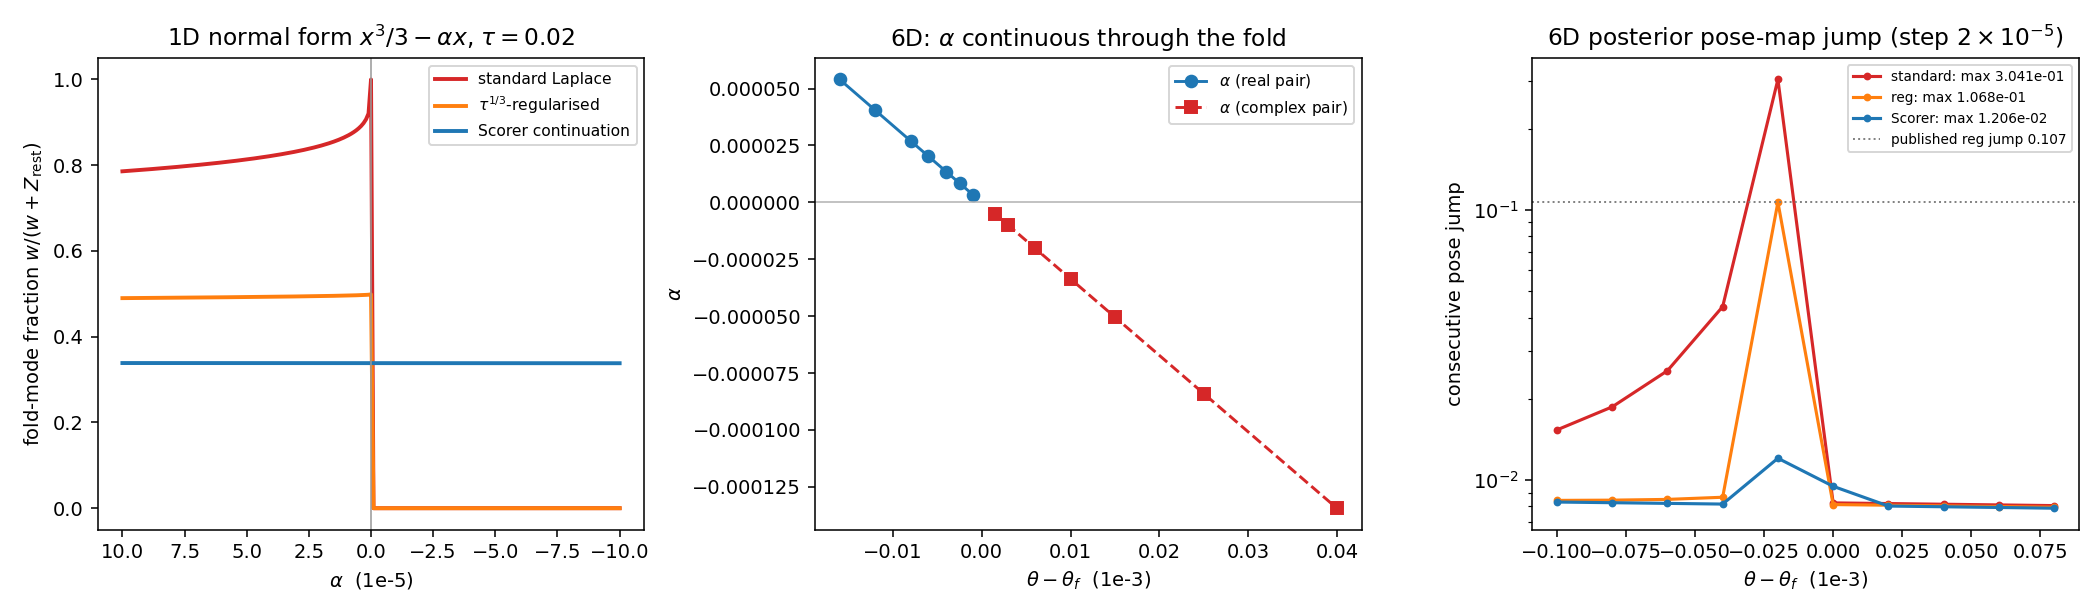
\includegraphics[width=0.80\textwidth]{scorer_fold.png}
\caption{The Scorer continuation at a fold. \textbf{Left:} the 1D normal form $x^3/3-\alpha x$ at $\tau=0.02$; the fold-mode weight fraction is discontinuous for the standard Laplace sum, jumps from $0.4959$ to $0$ for the $\tau^{1/3}$-regularised volume factor, and is continuous ($0.33838\to0.33834$) for the Scorer continuation. \textbf{Middle:} the 6D fold at $\theta_f=1.3185\times10^{-3}$; the invariant $\alpha$ is tracked through the fold, continuous across the real-pair/complex-pair switch. \textbf{Right:} the largest consecutive posterior pose jump against $\theta-\theta_f$: the standard map spikes to $3.04\times10^{-1}$, the regularised one to $1.07\times10^{-1}$, and the Scorer continuation peaks at $1.21\times10^{-2}$, at the smooth-map derivative scale.}
\label{fig:scorer}
\end{figure*}

The continuity claim is tested by grid refinement (staggered grids, half-width $10^{-4}$, step $d\in\{4\times10^{-5},\ldots,2.5\times10^{-6}\}$): the Scorer \emph{jump/d} stays $404.3,404.2,404.0,403.7,403.3$ over a $16\times$ range of $d$ (no numerical floor at $d=2.5\times10^{-6}$), whereas the standard map's \emph{jump/d} grows from $7.6\times10^{3}$ to $2.1\times10^{5}$ and the regularised one from $2.7\times10^{3}$ to $4.4\times10^{4}$ (a constant step). The fold neighbourhood therefore requires the Scorer continuation, or a local numerical integral over the merging pair, for a continuity claim.



\subsection{Future work}

Extending the evaluation to a learned front-end, to detector-level ADD(-S)/ADD-S AUC on LINEMOD/LINEMOD-Occlusion and to UTIAS In-The-Dark, and comparing against SDPR and EPro-PnP, are left for future work. A per-instance certified real-root count, a batched GPU forward, learned temperature calibration and third-derivative contraction for the full Laplace KL are the natural next steps.

\section{Conclusion}\label{sec:conclusion}

We have presented \textsc{Laplace-QPEPLayer}, a differentiable pose layer that combines the quaternion algebra of QPEP with a $3\times3$ Riemannian implicit differentiation and a multi-modal Laplace posterior. The theoretical core is an exact orthogonal bridge between the rotation lift and the Veronese embedding, a proof that the 21 standard $SO(3)$ constraints span the degree-two Veronese ideal, a certified Choi--Lam gap instance for the rotation subproblem, a three-part theorem relating the $10\times10$ relaxation to the released $13\times13$ one, and a closed-form backward pass with antipodal invariance. The probabilistic core is an exact translation integral and an analytic Laplace sum over all enumerated rotation minima, with explicit error order and failure modes. The design is deliberately narrow and its claims are scoped: no SDP lift at inference, no Monte Carlo sampling, no inequality constraints, no outlier kernel.

Section~\ref{sec:experiments} reports the experiments that are complete: the synthetic 6D branch-crossing benchmark (with an FD-step study, a measured fold, a fold theory and a timing/batching study), the 1D exact-posterior checks, the certificate and Jacobian verification, the ten-vs-thirteen SDP analysis (proved full-20D equivalence, proved and measured upstream looseness, and the 6-point physical separation), and a real-data LINEMOD two-mode study with a pose-error/ADD-S proxy and forward/local (classical PnP, Theseus) references.

The real-data result is a trade, not an accuracy win: the hard argmin is accurate at the near-ties (at the level of a classical EPnP/SQPNP, median $2.06^\circ$ and $3.7$ mm ADD-S) while the Laplace mean is biased toward the flip (median $44.24^\circ$ and $13.9$ mm ADD-S, paired bias $+36.9^\circ$), and the earlier $58.3^\circ$ figure was the unprojected 9-vector mean, not a rotation error. The layer buys a deterministic, sampling-free gradient that is smooth at branch crossings; it pays for that gradient in pose accuracy precisely on the frames where two modes are near-tied.

What remains is the real-image accuracy step: a learned front-end and the detector-level ADD(-S)/ADD-S AUC benchmark on LINEMOD/LINEMOD-Occlusion, the UTIAS In-The-Dark pipeline, the SDPR and EPro-PnP comparisons, a per-instance certified real-root count, and a batched (GPU) forward. None of these is claimed here, and every reported number is tagged with its evidence level in Table~\ref{tab:claimmap}.


\balance
\bibliographystyle{IEEEtran}
\bibliography{refs}

\end{document}
